\documentclass[11pt, a4paper]{report}
\makeatletter
\def\input@path{{../}}
\makeatother
% longtable before styling.sty (arydshln) — required for Paul’s longtable + \hline
\usepackage{longtable}
\usepackage{xspace}
\usepackage{rotating}
\usepackage{styling}
% styling.sty no longer loads biblatex (Toby commented it out so he can configure it himself).
\usepackage[backend=biber, style=numeric, sorting=none]{biblatex}
\DefineBibliographyStrings{english}{bibliography = {References}}
\providecommand{\contribution}[1]{\medskip\noindent\textbf{Section Contribution: #1}\par}
\usepackage{xurl}
\usepackage{multicol}
\usepackage{tocloft}
\setlength{\cftbeforetoctitleskip}{0pt}
\setlength{\cftaftertoctitleskip}{6pt}
\usepackage{tabularx}
\usepackage{array}

\numberwithin{equation}{section}

\addbibresource{../TobyMcConnell/Business/references.bib}
\addbibresource{../PaulVogelberg/Business/references.bib}
\addbibresource{../MichaelZiyangXing/references_eem_design.bib}
\addbibresource{yuze_business_references.bib}
\addbibresource{../HarryEmes/Business/references.bib}

\defbibnote{urlcheck}{All URLs were last accessed and verified on 01/04/2026.}

% Financial headline numbers for Harry's chapter (same as standalone Business/main.tex).
\newcommand{\yOneRevenue}{\pounds300k\xspace}
\newcommand{\yFiveRevenue}{\pounds2.1M\xspace}
\newcommand{\yFiveEbit}{\pounds0.4M\xspace}
\newcommand{\breakEvenYear}{Y4\xspace}
\newcommand{\breakEvenDays}{122\xspace}
\newcommand{\contributionMargin}{\pounds5,650\xspace}
\newcommand{\seedRound}{\pounds1.0M\xspace}
\newcommand{\seriesARound}{\pounds1.5M\xspace}
\newcommand{\totalRaise}{\pounds2.5M\xspace}
\newcommand{\capexPerVehicle}{\pounds310k\xspace}
\newcommand{\totalCapex}{\pounds0.98M\xspace}
\newcommand{\fixedOpexYOne}{\pounds538k\xspace}
\newcommand{\ltv}{\pounds126k\xspace}
\newcommand{\cac}{\pounds12k\xspace}
\newcommand{\ltvCac}{10.5\ensuremath{\times}\xspace}
\newcommand{\paybackMonths}{3.4\xspace}
\newcommand{\npvBase}{\pounds1.32M\xspace}
\newcommand{\npvHurdle}{\pounds0.97M\xspace}
\newcommand{\irr}{55.2\%\xspace}
\newcommand{\terminalValue}{\pounds5.2M\xspace}
\newcommand{\downtimeBreak}{$>30\%$\xspace}
\newcommand{\inversionCrossover}{Y2\xspace}


\title{Tracy --- Combined Business Report \\ Formula Student Acceleration Event}
\author{Toby McConnell, Paul Vogelberg, Ziyang Xing, Yuze Jiang, Harry Emes}
\date{\today}

\begin{document}

\pagenumbering{gobble}

\maketitle
\newpage

\pagenumbering{arabic}
\setcounter{page}{1}

\tableofcontents
\newpage

\begin{refsection}
\graphicspath{{../TobyMcConnell/Business/}}
\input{../TobyMcConnell/Business/toby_business_body}
\end{refsection}

\begin{refsection}
\graphicspath{{../PaulVogelberg/Business/}}
\chapterauthor{Strategy \& Stakeholder Analysis}{Paul Vogelberg}
\contribution{Paul Vogelberg}

\section{Introduction to the Strategic Pivot}

The UK Connected and Automated Mobility (CAM) sector faces a critical simulation-to-reality gap; regulators and insurers demand exhaustive physical edge-case validation before approving autonomous deployments, yet Original Equipment Manufacturers (OEMs) lack the agile hardware to safely execute these collisions. To address this bottleneck, our enterprise executes a foundational strategic manoeuvre: pivoting from the development and sale of a physical engineering asset (the AEB Rabbit) to providing a comprehensive Testing-as-a-Service (TaaS) platform. This allows autonomous vehicle (AV) developers to access high-fidelity, physical validation data without bearing the cost of maintaining their own target fleets.

This service model is enabled by our vehicle's specialised engineering architecture. Designed for rapid acceleration rather than cruising, the AEB Rabbit utilises a supercapacitor energy storage system to execute repeatable,  les than 10-second "panic" manoeuvres that mimic erratic human behaviour. To guarantee the high track utilisation required for TaaS profitability, the platform employs a modular supply chain strategy. By standardising replaceable impact shells and maintaining a buffer of drivetrain components, the enterprise ensures swift track-side mechanical recovery following a severe collision, protecting operational throughput.

Strategically, our Go-To-Market plan bypasses individual OEM bureaucratic delays by natively integrating the AEB Rabbit directly into established CAM Testbed UK facilities. Here, the enterprise serves as an ethical and legal buffer for AV developers. By operating strictly within defined Operational Design Domains (PAS 1883), governed by Safety Management Systems (PAS 1881), and providing immutable "black box" telemetry (PAS 1882), we absorb the physical risks of extreme edge-case testing. This provides the undeniable empirical evidence required by insurers and regulators to safely determine liability in a post-human-driver landscape.

Finally, this enterprise achieves rigorous environmental alignment without compromising commercial viability. At the macro level, the TaaS model operates as a Use/Result-Oriented Product-Service System (PSS), aggregating industry demand and preventing redundant OEM hardware manufacturing. Because the enterprise retains asset ownership under this model, we are financially incentivised to execute the 9R Circular Economy Framework. Sustainability is actively achieved through inherited lifecycle extension: utilising high-duty cycle supercapacitors, instituting drivetrain remanufacturing loops, and deploying recyclable Expanded Polypropylene (EPP) sacrificial shells to drastically reduce the operation's embodied carbon.

\section{Macro-Environmental Dynamics and the UK Ecosystem}

Our strategy leverages the government's investment focus, as outlined in the Zenzic UK CAM Roadmap, and capitalises on established CAM Testbed facilities.

\subsection{The Zenzic UK CAM Roadmap}

The most critical macro-environmental tool available for this analysis is the UK Connected and Automated Mobility (CAM) Roadmap to 2035, coordinated by Zenzic, a joint venture between UK industry and government \cite{zenzic_about}. The Roadmap acts as a comprehensive vision of the path required to create scalable solutions and bring CAM technologies to reality.

According to the executive summary \cite[p.~5,11,14]{cracknell_2023}, despite aggressive timelines to deploy self-driving vehicles by 2025, the UK AV sector is currently bottlenecked by a lack of physical, real-world validation. Regulators are hesitant to approve deployments without overwhelming proof of safety, and OEMs are concerned that a single public incident will derail their progress. The industry cannot scale until it can rigorously and safely physically test edge-cases.

Our testing vehicles provide the critical, physical validation layer required to bridge the gap between simulation and public deployment. We allow our clients to safely generate the hard data needed to satisfy regulators, achieve pre-certification, and protect their brand reputation from public accidents.

The total addressable market is expanding rapidly due to acute global labour shortages in freight, logistics, and public transport \cite[p.~6]{wef_2021}. Because operators are forced to adopt No-User-in-Charge (NUiC) vehicles to survive, OEMs are scaling their platforms faster than ever to meet this structural deficit \cite[p.~9,11,17]{cracknell_2023}. Every new platform and iteration requires exhaustive physical testing, creating a recurring, high-volume demand for our validation equipment.  
This venture is strategically aligned with the Centre for Connected and Autonomous Vehicles' (CCAV) ongoing Automated Vehicles Act implementation programme \cite{lawcom_avs_2024}, which fundamentally transitions the UK from regulatory theory into active commercial deployment % [Paul Vogelberg: Source also for this?]
. Concurrently, the Zenzic roadmap identifies the rapid acceleration of the domestic CAM supply chain as a primary macro-environmental driver for the sector \cite[p.~9,10,19]{cracknell_2023}. As the government actively seeks to build a world-class, sovereign CAM ecosystem with a strict legislative emphasis on physical safety assurance, our enterprise is ideally positioned to capture targeted grant funding. By aligning our business with the criteria of active government initiatives, specifically the £150 million CAM Pathfinder Programme to accelerate commercial market readiness \cite{pockney_2026}, we can leverage state-sponsored funding to integrate our physical validation tools directly into the UK's deployment infrastructure.

\subsection{Utilising CAM Testbed UK}

The UK offers a highly concentrated target market through 'CAM Testbed UK', a unified network of world-leading physical and virtual testbeds. Because safety-critical edge cases occur rarely and are dangerous to replicate in real-world traffic, developers cannot rely on waiting for them to naturally occur on public roads \cite[p.~12]{chen_2024}. Our vehicles solve this by allowing test engineers to repeatedly and safely recreate high-stakes, erratic scenarios in controlled environments. This rigorous scenario-based testing directly assists OEMs in meeting the BSI PAS 1881 standard to reduce testing risks to a level that is as low as reasonably practicable (ALARP) \cite[p.~1]{pas1881}, thereby fortifying their Operational Safety Case for regulatory approval.

Our system acts as the essential physical ground-truth required to validate the UK's investments in virtual simulation. Our product enables state-of-the-art facilities to correlate their virtual 'digital-twin' testing with real-world sensor data. Instead of focusing on targeting individual OEMs, with a heavy customer acquisition cost and prolonged procurement cycle, our strategy natively integrates the platform into the service offerings of centralised CAM Testbed facilities. This positioning establishes the enterprise as an indispensable, embedded supplier to the global testing hubs where the entire autonomous mobility industry already meets.

There is an established, proven precedent of demand within the CAM Testbed UK network for our precise technology. For instance, during the recent £5.8M project at the Culham Science Centre (a CAM Testbed UK facility), the delivery partners explicitly utilised government grant funding to purchase a motorised pedestrian dummy to increase their safety testing options \cite[p.~2]{culham_2024}. While these testbeds are currently investing in low-speed pedestrian targets, our TaaS model builds upon this precedent by filling the unaddressed, high-value gap for highly dynamic, high-mass vehicular targets. Our business is perfectly timed to capture this active, ongoing capital expenditure from UK testing facilities looking to maintain their global competitiveness % [Paul Vogelberg: Could explain how our service builds on this precedent. Maybe not precisely our service, need to clarify what our dummy represents in testing scenarios.]
.

\section{Manoeuvring to the Testing-as-a-Service (TaaS) Model}

As autonomous vehicle (AV) architectures evolve from modular pipelines to end-to-end (E2E) AI systems, an emerging market demand has surfaced for advanced dynamic testing. E2E systems frequently suffer from "causal confusion"—a critical failure mode where the model relies on spurious, false correlations that ultimately lead to catastrophic failures during real-world deployment \cite[p.~11-2]{chen_2024}. While developers primarily evaluate these models through offline, open-loop frameworks, the literature explicitly warns that such methods fail to measure a system's ability to recover from physical drift and do not provide conclusive evidence of safe driving behaviour \cite[p.~7]{chen_2024}. Consequently, rigorous, closed-loop dynamic benchmarking is not just beneficial, but fundamentally required.

Rather than relying on the traditional automotive diagnostic model that forces end-users into capital-intensive (CAPEX) hardware purchases, our enterprise addresses this critical evaluation gap through a TaaS delivery model. By strategically pivoting our physical engineering asset to a service-based approach, we equip client organisations, such as EV start-ups and OEM innovation divisions, % [Paul Vogelberg: insert reference to Toby's work]
with the dynamic, closed-loop physical environments required to expose and resolve causal confusion cost-effectively. Crucially, this model absorbs the operational burdens of hardware maintenance, infrastructure, and rapid technological obsolescence.

\subsection{Hardware Specialisation: The "Sprint" Advantage}

This TaaS strategy is explicitly necessitated by the unique mechanical profile of our adapted Formula Student (FS) architecture. The AEB Rabbit is not designed for a long duty cycle, but for short highly explosive acceleration, possessing a maximum power output lifetime of approximately 6 seconds per duty cycle % [Paul Vogelberg: source to engineering report figures here]
.

While this short operational runtime could render the vehicle unviable as a traditional commercial product for direct purchase, it is the performance envelope required to simulate extreme, dynamic edge cases (such as an erratic pedestrian darting into traffic, or a fast vehicle cutting across lanes). In our model, the client purchases the accurate data generated from a "panic" manoeuvre. Behind the scenes, our enterprise manages the operational duty cycle, using our accumulator system capability of rapid charging, reliable thermal management and consistent runs due to its supercapacitor architecture % [Paul Vogelberg: source to engineering report figures here]
, providing seamless and reliable value to the client.

\subsection{Full-Service Integration over Hardware Rental}

Our TaaS model fundamentally lowers this barrier to entry. By providing the self-propelled target, the trained safety operators, compliant with PAS 1884 \cite{pas1884}, and the continuous data-logging architecture, compliant with PAS 1882 \cite{pas1882}, we eliminate the need for our clients to train their own staff on complex, hazardous testing procedures. The client can simply dictate the conditions in which their automated vehicle should safely operate, the Operational Design Domain (ODD) parameters, and our enterprise can execute the required scenario to deliver the empirical data required for their safety cases.

\subsection{Supply Chain and Margin Defensibility}

The commercial viability of this TaaS model relies heavily on high utilisation rates and minimal track downtime. Because the AEB Rabbit will inevitably be subjected to physical impacts during edge-case validation, traditional testing rigs could suffer catastrophic, costly downtime.

Our platform utilises a modular architectural design, which ensures sustained profitability. By using standardised components and classifying them based on wear and collision-probability, our supply chain strategy can enable rapid, track-side mechanical recovery for the most likely repairs. This modularity prevents the total loss of the asset during a collision and isolates damage to affordable, replaceable outer components while protecting the high-value drivetrain. This strategic resilience secures consistent test throughput, directly underpinning the enterprise's robust operational expenditure (OPEX) forecasts and ensuring a predictable return on investment (ROI).

\section{Stakeholder Salience Identification}

\subsection{Introduction to the model}

\begin{figure}[h]
\centering
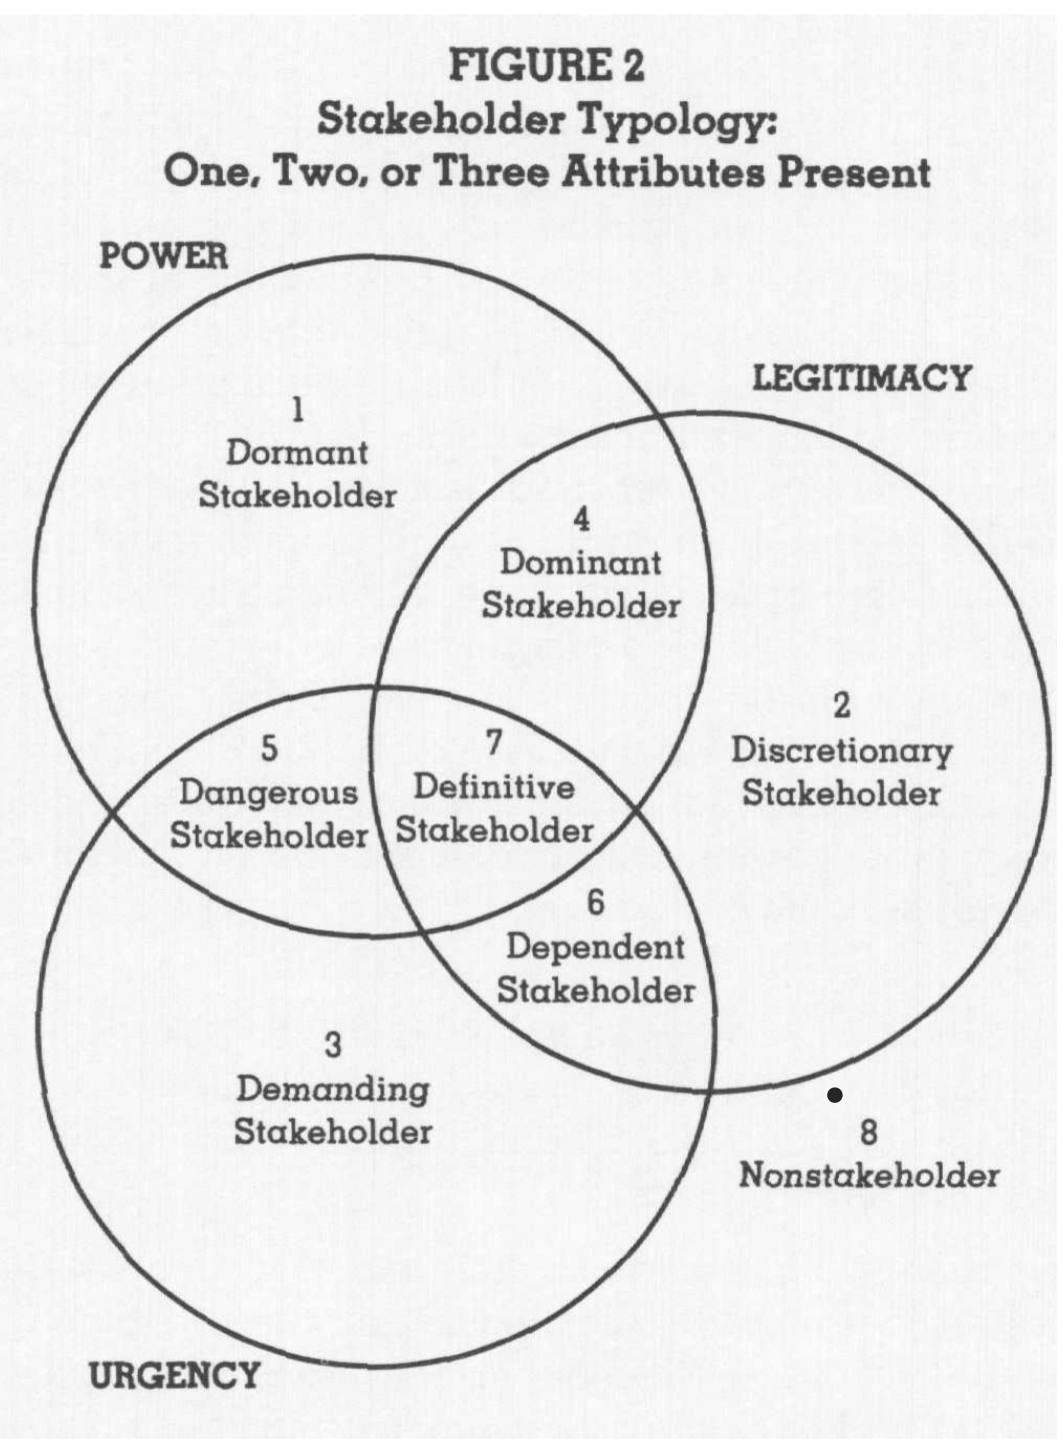
\includegraphics[width=0.6\textwidth]{figures/Figure1.jpeg}
\caption{Stakeholder Typology}
\end{figure}


While traditional matrices (such as RACI) map static operational responsibilities, the high-risk, heavily regulated nature of the CAM sector demands a dynamic framework for strategic resource allocation. The Mitchell et al. Stakeholder Salience Model \cite{mitchell_1997} is explicitly appropriate for this enterprise because it accounts for rapid, event-driven shifts in stakeholder priority and allows the management team to focus its limited engagement capital toward actors possessing two or more salience attributes. The model uses the triad: Power, Legitimacy, Urgency, for which a stakeholder can be assigned to a certain category using Figure 1.

In accordance with Proposition 1a, which asserts that 'stakeholder salience will be low where only one of the stakeholder attributes (power, legitimacy, and urgency) is perceived by managers to be present' \cite[p.~874]{mitchell_1997}, this report focuses its active engagement strategy on stakeholders possessing two or more of these attributes.

For every such class, the applicable stakeholders are given and the reasoning is explained:

\begin{itemize}
  \item Definitive Stakeholders - Insurers \& Testbed Operators: these actors possess all three attributes. Insurers hold financial power and legal legitimacy over operations, while their need for immediate post-incident data drives high urgency. Similarly, testbed operators have the power and legitimacy to halt trials instantly to protect their track's safety. Whilst the possibility of utilising OEMs' testing facilities exists, our market analyse shows that we should focus on EV start-ups and OEM innovation divisions.
  \item Dominant Stakeholders - Regulators \& Highway Authorities: entities such as CCAV hold ultimate regulatory power and legitimacy but generally exhibit lower urgency during day-to-day closed-track testing % [Paul Vogelberg: find source]
, as under Mitchell's theory, their urgency is typically event-driven and only spikes post-incident, provided compliance is maintained.
  \item Dependent Stakeholders - General Public: this group hold high moral legitimacy and urgency regarding their physical safety, but lack the direct power to enforce testing protocols, relying instead on our internal ethics governance.
  \item Dangerous Stakeholders - Cyber-Threat Actors: whilst this actor does not possess any legitimacy, it has both power and urgency to maliciously obtain valuable data or disrupt the service the enterprise is offering to their competitors.
\end{itemize}

\subsection{Applying the model}

For each stakeholder mentioned above, the salience class, alongside the value exchange provided and their respective compliance mechanism, split between the R\&D phase and the Commercial phase (if different, otherwise combined), are given in Table 1.


\begin{longtable}{|>{\doublespacing\arraybackslash}p{0.14\linewidth}|>{\doublespacing\arraybackslash}p{0.16\linewidth}|>{\doublespacing\arraybackslash}p{0.24\linewidth}|>{\doublespacing\arraybackslash}p{0.24\linewidth}|>{\doublespacing\arraybackslash}p{0.12\linewidth}|}
\caption{Strategic Engagement and Value Exchange Matrix} \\
\hline
\textbf{Stakeholder Group} & \textbf{Salience Class} & \multicolumn{2}{c|}{\textbf{The Value Exchange}} & \textbf{Compliance Mechanism} \\
\cline{3-4}
 & & \textbf{Need} & \textbf{Solution} & \\
\hline
\endfirsthead
\multicolumn{5}{c}
{{\bfseries \tablename\ \thetable{} -- continued from previous page}} \\
\hline
\textbf{Stakeholder Group} & \textbf{Salience Class} & \multicolumn{2}{c|}{\textbf{The Value Exchange}} & \textbf{Compliance Mechanism} \\
\cline{3-4}
 & & \textbf{Need} & \textbf{Solution} & \\
\hline
\endhead
\hline \multicolumn{5}{|r|}{{Continued on next page}} \\ \hline
\endfoot
\hline
\endlastfoot
Testbed Operators & Definitive in R\&D & Guarantee that the experimental prototype will not destroy track infrastructure. & Extreme transparency and rigorous safety mitigation plans. & PAS 1881 \cite{pas1881} SMS \\
\cline{2-5}
 & Definitive in Commercial & Attract top AV developers to rent their tracks. & We provide a highly integrated, value-add service that brings clients directly to their facility. & Modular Supply Chain \\
\hline
AV Start-ups \& OEMs & Discretionary (Latent) in R\&D & Assurance that the conceptual target will meet their AI requirements. & Market-fit validation and technical alignment. & PAS 1883 \cite{pas1883} (ODD Taxonomy) \\
\cline{2-5}
 & Definitive in Commercial & Capital-efficient, rapid edge-case validation. & We absorb CAPEX and hardware maintenance, delivering on-demand testing data. & \\
\hline
Component Suppliers & Definitive in R\&D & Proof of engineering viability for custom parts. & Custom tuning feedback and baseline component testing. & Engineering Service Legal Agreements \\
\cline{2-5}
 & Dominant (Urgency drops) in Commercial & Predictable, high-volume recurring revenue. & Long-term purchase orders to maintain our modular inventory buffer. & PAS 1881 \cite{pas1881} (Maintenance) \\
\hline
Insurers \& Investigators & Definitive & Irrefutable proof of liability during and after collisions. & We absorb the ambiguity of crashes by acting as an incorruptible data proxy. & PAS 1882 \cite{pas1882} (Immutable ECU Logging) \\
\hline
Regulators (e.g., CCAV) & Dominant & Proof that autonomous systems are reaching ALARP safety standards. & We provide the physical scenario-testing required to generate their safety metrics. & PAS 1881 \cite{pas1881} (Formal Operational Safety Case % [Paul Vogelberg: What exactly is this?]
) \\
\hline
The Public \& VRUs & Dependent & Protection from immature, dangerous AV technology. & We act as their proxy, absorbing the physical impacts of edge-case testing. & Ethics Impact Assessments \\
\hline
Cyber-Threat Actors & Dangerous & Goal: Exploit systemic vulnerabilities for disruption or hijacking. & Mitigation: Defensive shielding and encrypted telemetry to ensure testing integrity. & PAS 1885 \cite{pas1885} (Cybersecurity Principles) \\
\hline
\end{longtable}


\subsection{Continuations to the model}

While Table 1 maps the salience of these groups, it is important to distinguish the structural nature of their power. Within our Dominant and Definitive categories, actors such as CCAV, Thatcham Research, and BSI operate explicitly as 'Stakekeepers' \cite[p.~121]{fassin_2009}. Unlike traditional stakeholders who hold direct financial investments in the enterprise, stakekeepers are independent regulatory and certification bodies. They possess absolute institutional legitimacy and the power to dictate market access, meaning our strategy must prioritise their compliance requirements as foundational, non-negotiable operational constraints.

The enterprise treats these attributes not as binary states, but as a continuum. Latent groups are subjected to continuous passive monitoring to ensure we anticipate any escalation in their urgency or power before they cross the threshold into definitive threats.

\section{User Personas}

\subsection{The CAM Testbed Operations Director (The Partner)}

\textit{Context: Facility leadership at a state-backed testing ground, such as UTAC Millbrook-Culham}.

\textbf{Role:} Director of Track Operations and Commercial Partnerships.

\textbf{Motivations \& End Goals:} Evaluated strictly on track utilisation metrics and facility safety records. Their primary goal is to attract tier-1 AV developers by offering the most reliable, cutting-edge physical testing infrastructure in Europe.

\textbf{Pains:} Unpredictable, bespoke test-target suppliers. When a client's custom testing dummy shatters during a high-speed impact, the track must be shut down for hours to clear hazardous debris. This destroys the daily testing schedule, forces the facility to issue refunds for lost time, and artificially caps their revenue.

\textbf{Decision Influence \& Value Exchange:} Controls the "approved vendor" list for the facility. By exclusively partnering with our TaaS platform, they guarantee their clients rapid trackside recovery times. Furthermore, by transferring operational liability to our PAS 1884-compliant safety staff \cite{pas1884}, we directly boost their facility's daily throughput and derisk their commercial operations, making us an indispensable embedded supplier.

\subsection{The Independent Liability Assessor (The Gatekeeper)}

\textit{Context: Technical safety auditor for an insurance intelligence body (e.g., Thatcham Research) or government regulator (e.g., CCAV)}.

\textbf{Role:} Lead Risk Analyst for Automated Driving Systems (ADS).

\textbf{Motivations \& End Goals:} Tasked with establishing legal fault in simulated edge-case crashes to build the foundation for commercial insurance policies. They need empirical, unassailable data to verify that a system has met the "as low as reasonably practicable" (ALARP) safety threshold before certifying it for public roads.

\textbf{Pains:} Competing narratives during track incidents. AV developers often blame testing equipment or track conditions for edge-case failures rather than their own algorithms. This ambiguity makes it impossible for assessors to confidently price risk premiums or assign legal liability.

\textbf{Decision Influence \& Value Exchange:} Holds the ultimate veto over a vehicle's public road certification. By utilising our dummy vehicle's Electronic Control Unit (ECU) in compliance with PAS 1882 \cite{pas1882}, our platform provides them with an incorruptible, third-party "black box." We deliver objective telemetry that is completely independent of the OEM, solving their core data-integrity problem and incentivising them to mandate our platform for future Operational Safety Cases.

\section{Integrated Strategy for Ethics, Liability, and Safety Assurance}

The UK Automated Vehicles Act 2024 fundamentally shifts legal liability away from human drivers and onto the corporate developers \cite{lawcom_avs_2024}. In this environment, ethical obligations, legal liability, and safety assurance cannot be treated as isolated topics; they are inextricably linked. Our strategy navigates this complex web by positioning our hardware as the critical compliance tool across three integrated fronts:

\subsection{The Ethical Safety Buffer}

The industry faces a moral imperative to deploy life-saving AV technology, but balancing this with the severe risks of high-speed validation testing presents a profound ethical dilemma. Industry standards, such as BSI PAS 1881 \cite{pas1881}, mandate that public welfare must be protected and all operational risks reduced to a level that is "as low as reasonably practicable" (ALARP).

Our testing platform serves as an ethical and safety buffer. By allowing developers to conduct hazardous fault injection testing and edge-case validation within strictly defined Operational Design Domains (ODD) compliant with PAS 1883 \cite{pas1883}, we absorb their physical risk. This ensures the public is never subjected to the dangers of immature AV systems, fulfilling the ethical impact assessment requirements of PAS 1881 \cite{pas1881} while establishing the foundation for the client's Operational Safety Case. Furthermore, by providing an affordable TaaS platform, we lower the barrier-to-entry to testing, elevating the overall safety baseline of the industry beyond just the incumbent manufacturers.

\subsection{Liability Demarcation through Data Transparency}

Under the UK Law Commission's framework, our clients (operating as ASDEs) assume full legal responsibility for their vehicle's dynamic driving behaviour when their automated driving system (ADS) is engaged \cite{lawcom_avs_2024}. However, during physical edge-case validation, collisions are an expected outcome. To protect our enterprise from unwarranted fault attribution and circumnavigate the ambiguity of high-speed collisions, insurers and legal investigators require unhindered access to telemetry \cite{thatcham_2026}. Therefore, our strategy utilises the dummy vehicle's Electronic Control Unit (ECU) to provide continuous, high-fidelity data logging in compliance with PAS 1882 \cite{pas1882}. Acting as an incorruptible "black box," this system creates an immutable record of our hardware's telemetry. This transparency creates a clear demarcation of liability, ensuring that if an incident occurs while our equipment operates within its defined parameters, legal and financial responsibility falls definitively on the ASDE's algorithmic failure, thereby shielding our enterprise from unwarranted exposure.

\subsection{Algorithmic Bias, Cybersecurity, and Continuous Learning}

Safety and legal compliance are not static achievements. As testbeds and vehicles become highly interconnected nodes, insurers and regulators highlight systemic vulnerabilities, such as algorithmic bias and cyber-threats, as primary risk factors.

While the enterprise does not develop the internal AI algorithms of client vehicles, it is fundamentally responsible for the physical environments used to validate them. A critical systemic vulnerability in AV development is algorithmic "overfitting", where autonomous systems are trained exclusively against predictable, compliant traffic patterns and uniform vehicle shapes. To mitigate this, our platform institutes strict governance over physical scenario curation. By deploying modular target shells that replicate both a comprehensive matrix of vehicular geometries and high-dynamic, erratic behaviours, the enterprise prevents AVs from being validated in an artificially sanitised environment. This robust scenario diversity directly supports the UK Law Commission’s (2022) mandate that ASDEs must prove their systems can drive safely and legally across all foreseeable traffic conditions before public deployment \cite[pp.~49, 81--82, 87]{lawcom_2022}, thereby fortifying the client’s Operational Safety Case under PAS 1881 \cite{pas1881}.

To protect systemic integrity, our platform must align with PAS 1885 \cite{pas1885} cybersecurity principles, utilising encrypted communication protocols to prevent unauthorised software modifications or remote hijacking during coordinated manoeuvres.

Finally, all these elements are governed by a PAS 1881-compliant Safety Management System (SMS) \cite{pas1881}. By treating our safety cases as "live documents", any track near-misses or unexpected component behaviours are immediately fed back into a mandatory change-control loop, ensuring continuous operational improvement and ongoing regulatory compliance.

\section{Sustainability, Lifecycle, and the Circular Economy}

In the automotive sector, traditional Life Cycle Assessments (LCA) frequently rely on methodologies that weight tailpipe greenhouse gas emissions against the energy grid mix. However, for a fully electric, TaaS platform, the operational use-phase is effectively zero-emission. Because almost half of an EV's life cycle Global Warming Potential (GWP) is locked into its manufacturing \cite[p.~56]{hawkins_2013}, the strategic sustainability focus must pivot sharply away from operational emissions. To combat this production-heavy footprint, the report mandates "effective recycling programs and improved EV lifetimes" \cite[p.~61]{hawkins_2013}. Consequently, the enterprise directly operationalises these mandates by deploying a Product-Service System (PSS) framework to structurally extend the vehicle's lifespan, whilst utilising the 9R Circular Economy framework to execute closed-loop recycling, thereby reducing the environmental impact of autonomous validation to a level that is as low as reasonably practicable (ALARP).

\subsection{Product-Service Systems (PSS) Framework}

At the macro-business level, the enterprise's Testing-as-a-Service (TaaS) model operates strictly as a Result-Oriented Product-Service System (PSS). Specifically, it aligns with the classification of Activity Management and Outsourcing (Category 6) \cite[p.~254]{tukker}. By operating this centralised PSS model at established UK testbeds, we prevent multiple of our potential clients from needlessly extracting raw materials to manufacture and maintain their own low-utilisation testing fleets.

\subsection{The 9R Framework Application}

To achieve absolute alignment between environmental sustainability and commercial efficiency, the enterprise governs its lifecycle strategy through the 9R Circular Economy Framework \cite[p.~5]{potting_2017}. Because asset ownership is retained under the TaaS model, we are financially incentivised to maximise hardware lifespan. At the macro-level, this overarching Product-Service System (PSS) successfully executes the framework's highest tiers-Smarter product use and manufacture (R0-R2)-by refusing redundant OEM manufacturing and reducing overall material extraction across the industry.

However, at the micro-level, we face a critical engineering constraint: the reliance on the foundational Formula Student (FS) vehicle architecture. Because the base chassis and drivetrain materials are predetermined by this inherited design, the enterprise cannot optimise the platform's initial embodied carbon. To counter this, we deploy a modular hardware strategy designed to keep inherited materials at their highest utility despite the intense mechanical stress and frequent collisions of track testing. Consequently, our hardware management is categorised across three core subsystems, mapping directly to the framework's subsequent mandates to Extend lifespan (R3-R7) and ensure the Useful application of materials (R8-R9):

- Energy Storage (Extend Lifespan: R3 Reuse \& R7 Repurpose): The inherited design provides a massive environmental advantage by utilising a supercapacitor architecture rather than traditional Lithium-ion battery packs, which rely on heavily mined rare-earth metals and suffer high chemical degradation under extreme discharge rates. Supercapacitors possess an exceptional cycle life (often exceeding one million cycles), entirely bypassing the toxic end-of-life disposal challenges associated with Li-ion cells and ensuring the energy storage system outlasts the commercial lifecycle of the vehicle itself % [Paul Vogelberg: Add Eng report reference]
.
- The Drivetrain \& Chassis (Extend Lifespan: R4 Repair, R5 Refurbishment \& R6 Remanufacture): The platform will be subjected to intense mechanical stress through high-dynamic testing. By adopting a modular supply chain, high-value inherited components (such as electric motors and suspension linkages) can be managed through rigorous refurbishment and remanufacturing loops (R5/R6). Furthermore, the steel spaceframe allows for track-side welding and repair (R4), extending the life of the asset indefinitely and preventing the need to commission an entirely new chassis after minor track incidents. Consequently, in both the drivetrain and the chassis, sustainability is actively achieved through operational lifecycle extension.
- The Sacrificial Shell (Useful Application of Materials: R8 Recycle): The most significant hardware update to our initial design is the external target shell, our highest-wear component. The strategic plan explicitly rejects rigid composites, like carbon fibre, which utilise thermoset plastics. This material not only makes the component difficult to sustainably recycle, with the vast majority sent to landfills \cite[p.~2]{morici_2022}, but also introduces hazardous track debris through shattering. Instead, the enterprise specifies the use of Recycled Expanded Polypropylene (rEPP), which is a highly impact-absorbent, low-cost, and lightweight thermoplastic foam, already used in automotive pedestrian protection applications \cite[p.~1]{ramaswamy_2017}. Following a track collision, the shattered EPP shells can be cleanly collected, melted down, and re-extruded into brand new impact shells, establishing a perfectly closed, 100\% recyclable material loop (R9) (demonstrated in \cite{handtke_2024}).

\section{Strategic Limitations \& Cross-Functional Dependencies}

While our TaaS model effectively resolves the AV industry's simulation-to-reality gap, it introduces significant internal vulnerabilities. To ensure commercial viability, these strategic limitations must be actively managed through cross-functional engineering and financial integrations.

\subsection{Financial Exposure and Capital Intensity}

While the TaaS model provides immense operational flexibility for our clients by shifting their costs to OPEX, its primary strategic limitation is the structural inversion of our own capital expenditure (CAPEX). Unlike a traditional hardware sales model, our enterprise must absorb the massive upfront costs of manufacturing the AEB Rabbit fleet, securing testing infrastructure, and insuring the assets before a single billable testing hour is executed. To validate that this front-loaded financial exposure does not compromise enterprise solvency, our strategy relies entirely on the financial models (explored in % [Paul Vogelberg: add reference to Harry's financial report]
 the report) dictating the minimum utilisation rates required to sustain the TaaS strategy.

\subsection{Asset Ownership and the Maintenance Bottleneck}

Under the Product-Service System (PSS) framework, retaining asset ownership inherently transfers the financial risk of hardware failure from the client to the enterprise. Because our revenue generation is strictly tethered to track uptime, any collision damage that exceeds our forecasted repair windows directly erodes our margin defensibility. Furthermore, prolonged downtime threatens our relationships with our definitive stakeholders (i.e. the testbed operators). Consequently, the commercial execution of this strategy is fundamentally dependent on rigorous Supply Chain Planning % [Paul Vogelberg: add reference to David's section]
. The proposed modular inventory buffer and strict trackside recovery protocols act as the primary operational mitigation mechanism against our greatest commercial vulnerability.

\subsection{The Regulatory "Cold Start" Problem}

Finally, the strategy to natively integrate into established CAM Testbed UK facilities presents a regulatory "cold start" problem. Testbed operations directors and independent liability assessors (our "Stakekeepers") demand overwhelming empirical proof that our high-dynamic platform will not damage their permanent infrastructure or endanger personnel. However, we cannot capture market share until this safety is proven on a track. Overcoming this barrier requires rigorous, staged proof-of-concept testing prior to full commercial deployment. We mitigate this through the defined in the Design Requirements \& Prototype Planning % [Paul Vogelberg: add reference to Michael's work here]
, which ensure the platform systematically achieves the minimum viable safety thresholds required to secure initial testbed approval.




\printbibliography
\end{refsection}

\begin{refsection}
\graphicspath{{../MichaelZiyangXing/}}
% -----------------------------------------------------------------------------
% Compact preliminary EEM draft section for internal team review
% Project: UK-focused AEB test-carrier development from baseline EV chassis
% Target length: approximately 14--15 pages with styling.sty, figures, and references
% -----------------------------------------------------------------------------

\chapter{Commercially Driven Design Requirements and Prototype Planning}
\contribution{This chapter frames the design requirements and prototype plan for the autonomous emergency braking (AEB) test carrier from an Engineering Entrepreneurship and Management (EEM) perspective. It links technical requirements to UK customer needs, standards-led testing expectations, prototype-risk reduction, and commercialisation logic.}

\section{Purpose and commercial framing}

This chapter evaluates the design requirements and prototype plan for converting the team's baseline product, a lightweight and configurable electric vehicle (EV) chassis, into a high-dynamics autonomous emergency braking (AEB) test carrier. The proposed product direction is to prioritise vehicle-to-vehicle (V2V) AEB test cases, while retaining compatibility with less demanding tests such as pedestrian, cyclist, and low-speed obstacle scenarios. The design problem is therefore not only whether the vehicle can accelerate, brake, and follow a controlled path. It is whether these technical capabilities can become a credible and commercially useful testing asset for UK original equipment manufacturers (OEMs), proving grounds, connected and automated mobility (CAM) testbeds, advanced driver assistance system (ADAS) developers, and research organisations.

The chapter treats design requirements as market-facing requirements. Physical performance requirements determine which test cases the carrier can support. Experimental setup requirements determine whether the evidence produced is repeatable and usable. Standards and data requirements determine whether the prototype is credible in a professional UK testing environment. The prototype roadmap then shows how the team can begin with a low-cost exploratory platform, validate repeatability, demonstrate high-dynamics V2V capability, and finally package the system as a customer-ready demonstrator. This structure follows good practice observed in previous EEM project reports: clear customer segmentation, UK ecosystem framing, disciplined treatment of assumptions and financing, and operational realism around maintainability and downtime.

The scope is deliberately limited to the UK. EU and US regulatory pathways, including NHTSA-oriented expansion, are treated as future commercial scaling opportunities rather than immediate design drivers. This is appropriate for the current report because it keeps the design argument focused on UK customers, UK trial expectations, and relevant British Standards Institution (BSI) PAS documents. The central argument is that the test carrier should not be designed as a generic fast remote-controlled vehicle. It should be designed as a standards-aware, repeatable, data-producing test object that can support a future testing service or equipment offering.

\textbf{TODO: CONFIRM PROJECT-SPECIFIC SCOPE.} This draft assumes that the baseline EV chassis is available as a functioning or near-functioning platform and that the agreed market entry point is a high-dynamics AEB test carrier rather than a full autonomous driving vehicle. Before submission, this paragraph should be updated with the actual chassis status, the ownership of the baseline design, and the boundary between this EEM chapter and the engineering-design chapter.

\section{UK market need and customer problem}

\subsection{Why a physical AEB test carrier is useful}

AEB development increasingly uses simulation, software-in-the-loop testing, and controlled proving-ground experiments. Simulation is efficient for exploring large numbers of scenarios, but it cannot fully replace physical testing where perception, timing, actuation, tyres, surface condition, target presentation, and near-collision safety interact. For a customer, the value of a physical test carrier is therefore not only the vehicle itself. The value lies in producing repeatable, believable, and traceable evidence under controlled conditions.

The commercial opportunity sits between two extremes. Low-cost prototype platforms can be built quickly, but they often lack repeatability, data quality, safety documentation, and customer confidence. Premium active-safety test systems offer high capability, but they can be expensive, specialised, and difficult for smaller developers or research-led teams to access. The proposed AEB test carrier should occupy an intermediate position: a modular, lower-cost, UK standards-aware platform that first proves serious V2V testing capability and then matures towards a professional demonstrator.

\textbf{TODO: COLLECT MARKET EVIDENCE.} The final report should add at least two concrete evidence sources, such as stakeholder interviews, indicative supplier prices, published testbed-access rates, or CAM-sector reports. If exact costs cannot be obtained, the analysis should clearly state that it uses indicative cost bands rather than verified supplier quotations.

\subsection{Customer segments}

The first UK-focused commercialisation phase should target business-to-business customers rather than private consumers. The most relevant users are organisations that need to generate, validate, or sell AEB test evidence. Table~\ref{tab:customer_segments_compact} summarises the customer segments and their design implications.

\begin{table}[H]
\centering
\caption{Indicative UK customer segments and design implications.}
\label{tab:customer_segments_compact}
\begin{tabular}{p{0.20\textwidth} p{0.31\textwidth} p{0.37\textwidth}}
\toprule
\textbf{Segment} & \textbf{Primary need} & \textbf{Design implication} \\
\midrule
OEM validation teams & Repeatable V2V AEB evidence for internal development. & Prioritise acceleration, braking repeatability, trajectory control, logging, and reportable outputs. \\
\midrule
Proving grounds and CAM testbeds & Additional active-safety service capability. & Prioritise robust operation, fast reset, safety procedures, maintainability, and workflow integration. \\
\midrule
ADAS developers and Tier suppliers & Faster iteration between software changes and physical tests. & Prioritise modular scenarios, accessible data export, and lower operating cost. \\
\midrule
Research organisations & Affordable platform for controlled safety experiments. & Prioritise safe operating limits, instrumentation access, and transparent limitations. \\
\bottomrule
\end{tabular}
\end{table}

The shared customer problem is access to controlled physical validation without immediately taking on the full cost, complexity, and liability burden of premium target fleets. This makes the prototype plan commercially important. The team must not simply maximise technical ambition; it must decide which capabilities create customer confidence at each stage of development.

\subsection{UK policy and standards context}

The UK context strengthens the rationale because connected and automated mobility is an active national policy and investment area. The Automated Vehicles Act 2024 creates a legal framework for automated vehicles in Great Britain, while UK Government and CAM Testbed UK material presents automated mobility as a growth sector and testbed opportunity \parencite{automatedVehiclesAct2024,govukAVJobs2025,camTestbedUK}. The project should not claim that a university prototype is immediately compliant with commercial certification requirements. Instead, UK policy and standards should be used as design guidance: they show what a serious testing platform will eventually need to demonstrate.

For this report, the most relevant UK-facing references are PAS 1881 for operational safety, PAS 1882 for data collection and incident-investigation readiness, PAS 1883 and BS ISO 34503 for Operational Design Domain (ODD) definition, the Department for Transport automated vehicle trialling code of practice, ISO 22133 for test-object monitoring and control, and the ISO 19206 series for surrogate targets \parencite{bsiPAS1881,bsiPAS1882,bsiPAS1883,iso34503,dftTriallingCode,iso22133,iso19206series}. These sources do not all apply in the same way, but together they justify three design priorities: safe operation, repeatable tests, and traceable evidence.

\textbf{TODO: VERIFY VERSION-SENSITIVE STANDARDS.} Some standards are version-sensitive. Before submission, the team should confirm the exact current versions available through the university or BSI access, especially PAS 1881, PAS 1883, and ISO 22133. The report should avoid claiming formal compliance unless the corresponding evidence has been generated.

\begin{table}[H]
\centering
\caption{UK-focused standards and design implications.}
\label{tab:standards_design_compact}
\begin{tabular}{p{0.25\textwidth} p{0.61\textwidth}}
\toprule
\textbf{Reference} & \textbf{Implication for the AEB test-carrier project} \\
\midrule
PAS 1881 & Motivates safety-case thinking, operating limits, emergency procedures, change control, and monitoring of safety assumptions. \\
PAS 1882 & Motivates structured data capture, data retention, incident review, access control, and evidence preservation. \\
PAS 1883 / BS ISO 34503 & Motivates a clearly defined ODD for the prototype, including test environment, surface, speed range, target type, and weather limits. \\
DfT trialling guidance & Reinforces safety management, competent supervision, and responsible operation during public or semi-public trials. \\
ISO 22133 / ISO 19206 & Supports compatibility with active-safety test-object control and surrogate target expectations. \\
\bottomrule
\end{tabular}
\end{table}

\section{Design requirements as commercial requirements}

\subsection{Requirement logic}

The design requirements are organised into three lenses: physical performance, experimental setup, and standards/data readiness. This avoids presenting the carrier as a collection of unrelated technical specifications. Each lens answers a customer-facing question. First, can the platform execute the test cases that customers value? Second, can it repeat those tests reliably enough for engineering evidence? Third, can it produce data and documentation that a professional customer can trust?

\begin{table}[H]
\centering
\caption{Commercial interpretation of key design requirements.}
\label{tab:requirements_compact}
\begin{tabular}{p{0.18\textwidth} p{0.31\textwidth} p{0.24\textwidth} p{0.17\textwidth}}
\toprule
\textbf{Lens} & \textbf{Key points} & \textbf{Customer value} & \textbf{Example target} \\
\midrule
Physical performance & Acceleration, braking, top speed, payload, low-profile structure, and target compatibility. & Enables higher-value V2V AEB cases rather than only low-speed target motion. & 0--X km/h in $<$ X s; decel $>$ X m/s$^2$. \\
\midrule
Experimental setup & Repeatable speed, path, heading, scenario reset, emergency stop, and run-to-run consistency. & Reduces wasted test time and increases confidence that measured differences are caused by the vehicle under test. & Speed error $<$ $\pm$X km/h; lateral error $<$ $\pm$X m. \\
\midrule
Standards and data & Synchronised logging, scenario metadata, incident records, operating limits, and traceable reports. & Converts a moving carrier into professional test evidence. & Logging $>$ X Hz; time sync error $<$ X ms. \\
\bottomrule
\end{tabular}
\end{table}

\subsection{Physical performance}

The physical-performance requirements determine whether the platform can credibly support the chosen market position. A pedestrian-only target carrier can be relatively low speed and low acceleration, but V2V AEB scenarios require stronger longitudinal performance, stability, and control. The carrier should therefore be designed around measurable targets such as 0--X km/h acceleration time, maximum test speed of X km/h, braking deceleration above X m/s$^2$, payload capacity of X kg, and safe operation with a soft vehicle target mounted or towed.

These figures should not be treated as arbitrary engineering ambitions. They are commercial filters. If the chassis cannot reach the required dynamics, it may still be useful for low-speed research, but it will not support the differentiated value proposition of high-dynamics V2V AEB testing. Conversely, over-specifying the vehicle too early would increase cost before demand is validated. The correct approach is to define minimum performance thresholds for each prototype stage and tighten them only after early tests show the chassis can support further development.

\textbf{TODO: INSERT ACTUAL PERFORMANCE TARGETS.} Replace X values with measured or justified targets from the engineering team. The final report should state whether each target is an aspiration, a calculated requirement, or a measured prototype result.

\subsection{Experimental setup and repeatability}

Repeatability is the bridge between a technical prototype and a test product. The carrier must be able to execute the same scenario multiple times with controlled variation in speed, path, heading, acceleration, and timing. This is commercially important because testbed operators sell reliable test time. If the platform requires long manual setup, has high downtime, or produces inconsistent runs, its commercial value falls even if the hardware is impressive.

The experimental requirements should therefore include both test-quality and operational metrics. Test-quality metrics include path error below $\pm$X m, speed error below $\pm$X km/h, heading error below $\pm$X degrees, and repeatability over X repeated runs. Operational metrics include reset time below X minutes, number of runs per charge above X, repair time after minor contact below X minutes, and number of staff required per test day. These operational details connect engineering decisions to the EEM criteria because they affect cost, utilisation, and customer satisfaction.

\subsection{Standards, data, and evidence quality}

The standards/data lens converts motion into evidence. The platform should record sufficient data to reconstruct each run and explain the test context. A preliminary data-channel set should include timestamp, position, velocity, acceleration, yaw or heading, drive command, braking command, energy-store state, communications status, emergency-stop status, fault codes, scenario ID, operator, software version, weather condition, and any deviations from the planned test.

The logging frequency should be selected according to the fastest dynamics that need to be captured. In this draft, X Hz is used as a placeholder; the team should decide whether 100 Hz is technically achievable and commercially necessary for the later prototype. The report should be careful with wording. It can say that the data architecture is designed with standards-aware logging in mind, but it should not claim compliance until the sensors, synchronisation, storage, calibration, and data-processing chain have been validated.

\textbf{TODO: CONFIRM DATA ARCHITECTURE.} The final report should specify which channels are recorded at high frequency, which are recorded at lower frequency, how time synchronisation is achieved, and how raw logs are converted into customer-facing reports. If the early prototype cannot achieve the final logging target, present this as a staged limitation rather than a failure.

\section{Prototype roadmap: Explore, Validate, Demonstrate, Convince}

\subsection{Why staged prototyping is necessary}

The project begins with limited resources, uncertain customer demand, and unverified technical performance. A single attempt to build a customer-ready product from the beginning would create high financial and technical risk. A staged roadmap reduces this risk by creating decision gates. Each stage answers a clear question: can the chassis move safely; can it repeat a controlled test; can it demonstrate high-dynamics V2V value; and can it produce evidence that customers would trust?

\begin{figure}[H]
\centering
\fbox{\parbox{0.86\textwidth}{\centering\vspace{7mm}
\textbf{PLACEHOLDER FOR ROADMAP FIGURE}\par
A compact vertical figure should show: P0 Explore $\rightarrow$ P1 Validate $\rightarrow$ P2 Demonstrate $\rightarrow$ P3 Convince. Each stage should contain two or three short phrases. The style should match the dark-blue presentation theme.\vspace{7mm}}}
\caption{Staged prototype path from low-cost exploration to customer-ready proof.}
\label{fig:prototype_roadmap_compact}
\end{figure}

\subsection{Stage definitions}

P0, \textit{Explore}, should use the baseline EV chassis with the minimum modifications required for safe controlled motion. The purpose is to learn cheaply, not to impress customers. The expected evidence includes simple acceleration traces, braking traces, emergency-stop tests, video records, and operator feedback. If the chassis cannot meet a minimum motion envelope at P0, the team can pivot before investing in expensive sensors or target structures.

P1, \textit{Validate}, should convert the moving chassis into a repeatable experimental platform. The main additions are closed-loop velocity control, improved position or heading estimation, structured scenario setup, and reliable logging. The output should be a repeatability evidence pack showing, for example, that the vehicle can run a planned path at X km/h with speed error below $\pm$X km/h and lateral error below $\pm$X m over X repeated runs.

P2, \textit{Demonstrate}, should show the differentiated value proposition: high-dynamics V2V AEB testing. This stage should add soft vehicle target integration, a priority scenario library, stronger safety supervision, and enough performance to execute commercially interesting cases. Candidate cases include stationary target approach, moving target approach, braking target, crossing target, or low-speed cut-in scenarios. The exact scenario set should be chosen to match both customer interest and safe technical capability.

P3, \textit{Convince}, should package the prototype into a customer-ready demonstrator. This does not necessarily mean full commercial certification. It means that the prototype has the artefacts needed for a serious pilot discussion: operating manual, risk assessment, safety-case outline, scenario catalogue, data-export format, report template, maintenance plan, and costed service model. At this stage, the aim is not merely to show that the vehicle is fast; it is to reduce customer uncertainty.

\begin{table}[H]
\centering
\caption{Prototype stages, evidence outputs, and business decisions.}
\label{tab:prototype_stages_compact}
\begin{tabular}{p{0.14\textwidth} p{0.25\textwidth} p{0.29\textwidth} p{0.20\textwidth}}
\toprule
\textbf{Stage} & \textbf{Prototype focus} & \textbf{Evidence produced} & \textbf{Decision enabled} \\
\midrule
P0 Explore & Basic chassis motion and safe stop. & Feasibility video, acceleration/braking traces, failure notes. & Continue, redesign, or pivot. \\
P1 Validate & Repeatability, control, and logging. & Repeatability plots and structured logs. & Decide whether external demonstration is credible. \\
P2 Demonstrate & High-dynamics V2V scenarios. & Scenario videos, target integration, safety procedure. & Seek testbed or customer feedback. \\
P3 Convince & Customer-ready workflow and reports. & Report template, operating pack, risk pack, costed offer. & Launch pilot, lease trial, or service partnership. \\
\bottomrule
\end{tabular}
\end{table}

\textbf{TODO: INSERT CURRENT PROTOTYPE STATUS.} The final report should identify which stage the team has actually reached and which stages remain planned. If P0 or P1 tests have been completed, include measured performance, key failures, and lessons learned. If they have not been completed, the report should clearly describe them as planned decision gates.

\section{Value proposition and business model}

\subsection{Value proposition}

The proposed value proposition is a modular, lower-cost, UK standards-aware AEB test carrier that enables repeatable active-safety scenarios without requiring customers to immediately invest in a premium full-scale target system. Its initial differentiation should be practical rather than exaggerated: the platform should offer a credible route to V2V AEB testing, faster iteration, structured logs, and a development pathway that can be adapted to customer feedback.

For OEMs and ADAS developers, the value is additional physical evidence during development. For testbeds, the value is a possible new service capability. For research organisations, the value is an affordable and transparent platform for controlled experiments. Across these segments, the strongest commercial message is not simply low cost. It is lower cost combined with repeatability, safety awareness, and clear evidence outputs.

\subsection{Commercial model options}

Three business models are plausible. Direct product sale gives simple revenue but creates support and liability burdens. Leasing lowers customer entry cost and may suit testbeds that want equipment access without immediate purchase. Testing-as-a-Service gives the team more control over safety, maintenance, and data quality, but it requires staff time, site access, insurance, and operational planning. For the early UK phase, the most realistic route is likely prototype-led customer engagement followed by either a testbed partnership or a limited Testing-as-a-Service pilot.

\begin{table}[H]
\centering
\caption{Indicative business model comparison.}
\label{tab:business_model_compact}
\begin{tabular}{p{0.21\textwidth} p{0.29\textwidth} p{0.20\textwidth} p{0.20\textwidth}}
\toprule
\textbf{Model} & \textbf{Description} & \textbf{Strength} & \textbf{Limitation} \\
\midrule
Product sale & Sell the carrier hardware and support package. & Clear transaction and scalable if mature. & High support, warranty, and liability burden. \\
Leasing & Provide carrier access for a monthly or project fee. & Lowers customer entry cost. & Requires capital ownership and maintenance capacity. \\
Testing-as-a-Service & Operate the carrier for customers at a test site. & Controls quality and builds service revenue. & Requires staff, insurance, test-site access, and scheduling. \\
\bottomrule
\end{tabular}
\end{table}

\textbf{TODO: ADD COST AND PRICE ASSUMPTIONS.} The final report should include a simple cost model with indicative capital expenditure, operating expenditure, maintenance cost, staff cost, utilisation, and price per test day or pilot. If precise prices are unavailable, the analysis should present low/medium/high scenarios and explain the assumptions.

\section{Assumptions, risks, and limitations}

\subsection{Key assumptions}

The commercial argument depends on several assumptions. The report should state them explicitly rather than hiding them inside the narrative. The most important assumptions are that UK customers value lower-cost access to repeatable AEB testing, that the baseline chassis can meet the minimum high-dynamics envelope, that standards-aware logging increases customer confidence, and that a staged prototype path reduces financial risk.

\begin{table}[H]
\centering
\caption{Core assumptions and validation actions.}
\label{tab:assumptions_compact}
\begin{tabular}{p{0.36\textwidth} p{0.26\textwidth} p{0.27\textwidth}}
\toprule
\textbf{Assumption} & \textbf{Why it matters} & \textbf{How to test it} \\
\midrule
UK test operators want lower-cost AEB test capability. & Supports demand and positioning. & Interview testbeds, OEMs, and ADAS developers. \\
The baseline chassis can reach the required dynamics. & Supports the V2V value proposition. & Run P0/P1 acceleration, braking, and stability tests. \\
Customers value traceable logs and reports. & Supports standards-aware differentiation. & Show sample reports and collect feedback. \\
Staged prototyping reduces financial risk. & Supports funding and decision gates. & Review costs and evidence at each stage. \\
\bottomrule
\end{tabular}
\end{table}

\subsection{Risk management}

The main risks are technical, market, operational, safety, and commercial. Technical risk arises if the chassis cannot meet the acceleration, braking, stability, or payload requirements. Market risk arises if customers prefer established premium systems or if the lower-cost niche is smaller than expected. Operational risk arises from downtime, damaged target structures, battery or energy-store limitations, and manual setup burden. Safety risk is especially important because the prototype operates close to vehicles, targets, and test personnel. Commercial risk arises if the project cannot convert prototype evidence into a credible pilot or revenue model.

Mitigation should follow the staged roadmap. P0 and P1 reduce technical risk early. Customer interviews and testbed conversations reduce market risk before expensive P2 integration. Modular design, spare parts, and maintenance planning reduce operational risk. Emergency stop, geofencing, operating limits, competent supervision, and safety-case documentation reduce safety risk. A simple staged budget and business-model comparison reduce commercial risk.

\textbf{TODO: ADD TEAM RISK REGISTER.} The final report should include the team's actual risk register or a condensed version of it. Each risk should have a likelihood, impact, owner, mitigation, and residual risk rating if those are available.

\subsection{Limitations}

The proposed design and business plan have clear limitations. First, the prototype is not yet a certified commercial test system. Second, the UK-only scope improves focus but limits immediate international scalability. Third, performance targets remain provisional until validated by physical tests. Fourth, customer willingness to pay is assumed rather than proven. Fifth, standards are used as design guidance unless full compliance evidence is generated. Finally, the shift from low-speed target motion to high-dynamics V2V operation may require stronger mechanical design, more reliable control, and more robust safety systems than the baseline chassis currently provides.

Recognising these limitations strengthens rather than weakens the commercial case. It shows that the team understands the gap between a promising prototype and a sustainable product or service. The correct conclusion is therefore not that the design is already market-ready, but that the proposed roadmap gives a credible route for converting technical capability into customer evidence.

\section{Sustainability, ethics, IP, and conclusion}

Sustainability should be considered through the life cycle of the platform. An electric test carrier avoids local exhaust emissions during operation, but this does not make the project automatically sustainable. Battery sourcing, charging demand, tyre and brake wear, damaged target materials, electronic components, and end-of-life disposal should be considered. A modular repairable design can improve sustainability by extending platform life and reducing waste after minor impacts.

Ethical issues arise because AEB testing is safety-related. Poor testing could create false confidence in a vehicle system, while unsafe demonstrations could harm operators or damage equipment. The team should therefore communicate limitations clearly, avoid overstating compliance, and use conservative operating envelopes during early prototypes. Security and intellectual property also matter. Data logs may contain commercially sensitive customer information, while the control software, chassis modifications, and reporting workflow may contain protectable know-how. Access control, version management, and clear ownership of design files should be part of the prototype plan.

\textbf{TODO: CONFIRM IP AND DATA OWNERSHIP.} Before submission, the team should confirm who owns the baseline chassis design, software, data logs, and any modifications produced during the project. If customer demonstrations are planned, the report should explain how test data will be stored, shared, and protected.

This chapter has argued that the AEB test carrier should be developed through a commercially driven requirements process. The UK market context creates a plausible opportunity for a lower-cost, modular, standards-aware platform that can support repeatable active-safety testing. The requirements are therefore not only technical specifications; they are conditions for customer confidence. The staged roadmap from Explore to Validate, Demonstrate, and Convince reduces early financial risk while building towards a customer-ready evidence package. The project remains dependent on validation of performance, demand, cost, and safety assumptions, but the proposed plan provides a coherent route from an engineering prototype to a commercially meaningful UK testing proposition.


\printbibliography
\end{refsection}

\begin{refsection}
\graphicspath{{yuze_assets/}}
../Yuze Jiang/yuze_business_body.tex
\end{refsection}

% Shared compact chapter headings + list helpers for Harry's business chapter.
% Loaded by standalone main.tex and by CombinedBusiness before Harry's refsection.

\makeatletter
\renewcommand\chapter{\par%
  \thispagestyle{plain}%
  \global\@topnum\z@
  \@afterindentfalse
  \secdef\@chapter\@schapter}
\renewcommand{\@makechapterhead}[1]{%
  \vspace*{10pt}%
  {\parindent \z@ \raggedright \normalfont
    \ifnum \c@secnumdepth >\m@ne
      \Large\bfseries \@chapapp\ \thechapter: \ #1%
    \else
      \Large\bfseries #1%
    \fi
    \par\nobreak
    \vskip 8pt}}
\renewcommand{\@makeschapterhead}[1]{%
  \vspace*{10pt}%
  {\parindent \z@ \raggedright
    \normalfont
    \Large\bfseries #1\par\nobreak
    \vskip 8pt}}
\makeatother

\newenvironment{tightitemize}%
  {\begin{itemize}\setlength{\itemsep}{2pt}\setlength{\parskip}{0pt}\setlength{\topsep}{4pt}}%
  {\end{itemize}}
\newenvironment{tightenumerate}%
  {\begin{enumerate}\setlength{\itemsep}{2pt}\setlength{\parskip}{0pt}\setlength{\topsep}{4pt}}%
  {\end{enumerate}}


\begin{refsection}
\graphicspath{{../HarryEmes/Business/figures/}{../HarryEmes/Business/}}
% =====================================================================
\chapterauthor{Financial Analysis}{Harry Emes}
% =====================================================================

\noindent This chapter quantifies the five-year TaaS plan using one
driver-based Python model consistent with the engineering
chapter's sensitivity methodology~\cite{emes_engineering}: linked
capex, opex, and revenue; P\&L and free cash flow; break-even and one-at-a-time
sensitivities (Sections~\ref{sec:breakeven}--\ref{sec:business_sensitivity});
NPV/IRR (Section~\ref{sec:npv}); and downtime stress
(Section~\ref{sec:downtime}). Market sizing and day-rate inputs are carried over from
the market and competition material earlier in this report. Fleet-recovery and gatekeeper uptake assumptions align with the
preceding business chapters.

\medskip

\noindent \textbf{Headline financial evaluation}:

\begin{tightitemize}
  \item \textbf{CAPEX commitment:} \totalCapex over five years
        (\capexPerVehicle per vehicle $\times$ 3 vehicles +
        \pounds50\,k Y1 setup). Cumulative revenue first exceeds
        cumulative CAPEX in \inversionCrossover.
  \item \textbf{Five-year trajectory:} \yOneRevenue revenue $\to$
        \yFiveRevenue; break-even in \breakEvenYear at
        \breakEvenDays test days/year (contribution
        \contributionMargin per day).
  \item \textbf{Funding:} \seedRound seed + \seriesARound Series~A,
        total \totalRaise equity. Peak cumulative cash outflow
        occurs end-Y2 ($\sim$\pounds90\,k residual).
  \item \textbf{Capital return:} project NPV \npvBase at a 20\% VC
        discount rate, \npvHurdle at a 25\% hurdle rate, IRR \irr,
        all including a \terminalValue terminal value at $2.5\times$
        Y5 revenue.
  \item \textbf{Sensitivity:} day-rate and utilisation dominate; a
        $\pm 20\%$ swing in either drives $\sim$\pounds 270--370\,k
        in Y3 EBIT.
  \item \textbf{Downtime sensitivity:} NPV stays positive through
        \downtimeBreak unplanned fleet downtime, but Y5~EBIT turns
        negative once downtime exceeds $\sim$20\%. Fleet-maintenance
        protocols are therefore the single most binding execution
        dependency on the financial plan.
\end{tightitemize}

\noindent \textbf{Conclusion}: the TaaS financial structure clears
standard venture-capital thresholds in the base case and is
robust to adverse swings in the key commercial drivers
(Section~\ref{sec:business_sensitivity}).

% =====================================================================
\section{Key driver assumptions and their justification}
\label{ch:intro}
\label{sec:why_taas}
\label{sec:assumptions}
% =====================================================================

All headline figures come from one Python driver set; the bullets
below are the audit trail for the inputs that move the needle.

\paragraph{CAPEX and revenue drivers.} Per-vehicle build
\capexPerVehicle{} is five buckets (vehicle \pounds180\,k,
instrumentation \pounds60\,k, safety \pounds25\,k, trailer
\pounds30\,k, spares \pounds15\,k), aligned with the engineering
BOMs~\cite{mcconnell_engineering,xing_engineering,jiang_engineering,vogelberg_engineering}; Y1
\pounds50\,k workshop/data setup sits outside the per-vehicle line
for year-on-year comparability. Bronze/Silver/Gold day rates
\pounds6\,k/\pounds8\,k/\pounds10\,k are benchmarked to
AB~Dynamics, UTAC, HORIBA~MIRA, and AVL~\cite{abdynamics_ar2024,utac_facilities,horiba_brake,avl_profile};
tier prices are fixed and the blended rate rises only through
mix-shift (\pounds7.5\,k$\to$\pounds9.5\,k). Billable days per
vehicle 40/70/110/150/220 Y1--Y5 tie to the Market SOM
\cite{mcconnell_business} and reconcile \yFiveRevenue{} to
10--14\% of the \textdollar26\,M SOM developed in the market-sizing analysis earlier in this report.

\paragraph{Opex, variable cost, and tax.} Headcount uses Reed 2025
UK automotive mid-bands~\cite{reed_salaries_2025} with CEO at the
low end of the startup range; gross salaries carry a flat 20\%
on-cost (approx.\ 15\% employer NIC, 3\% auto-enrolment pension,
2\% misc.). Variable cost \pounds2{,}300/day Y1 splits tyres
\pounds800, transport \pounds600 (HMRC 45p/mile on a 200-mile
round trip, conservative vs.\ the 25p tail), crew \pounds400, wear
\pounds500. Fixed opex inflates 3\%/yr from CPIH
\cite{ons_cpi_2025} with hire step-ups at fleet events. Corporation
tax uses a flat 19\% from Y4~\cite{hmrc_corp_tax} rather than full
banding, consistent with the precision of the revenue forecast.

\paragraph{Capital return.} Discount rate 20\% (VC opportunity cost
\cite{brealey2020}); terminal value at peer-median $2.5\times$ Y5
revenue as in Section~\ref{sec:npv}
\cite{abdynamics_ar2024,damodaran2012,avl_profile}.
Section~\ref{sec:scenarios} stress-tests that terminal-heavy NPV.

% =====================================================================
\section{Cost structure, revenue model and five-year forecast}
\label{ch:cost_revenue}
% =====================================================================

% ---------------------------------------------------------------------
\subsection{CAPEX model: the cost of ownership the operator absorbs}
\label{sec:capex}
% ---------------------------------------------------------------------

The operator owns the fleet; the customer rents days. Every pound
of AEB~Rabbit capital therefore sits on our balance sheet, is
financed from equity until the business turns cash-positive, and is
recovered through the day-rate. Per-vehicle build is
\capexPerVehicle; the
Y1 setup adds \pounds50\,k in workshop fit-out and data-platform
infrastructure. Fleet growth (2nd vehicle in Y3, 3rd in Y5) drives
a further \pounds620\,k of capex over Y3--Y5. Total capex over the five-year
plan: \totalCapex.

\begin{figure}[H]
\centering
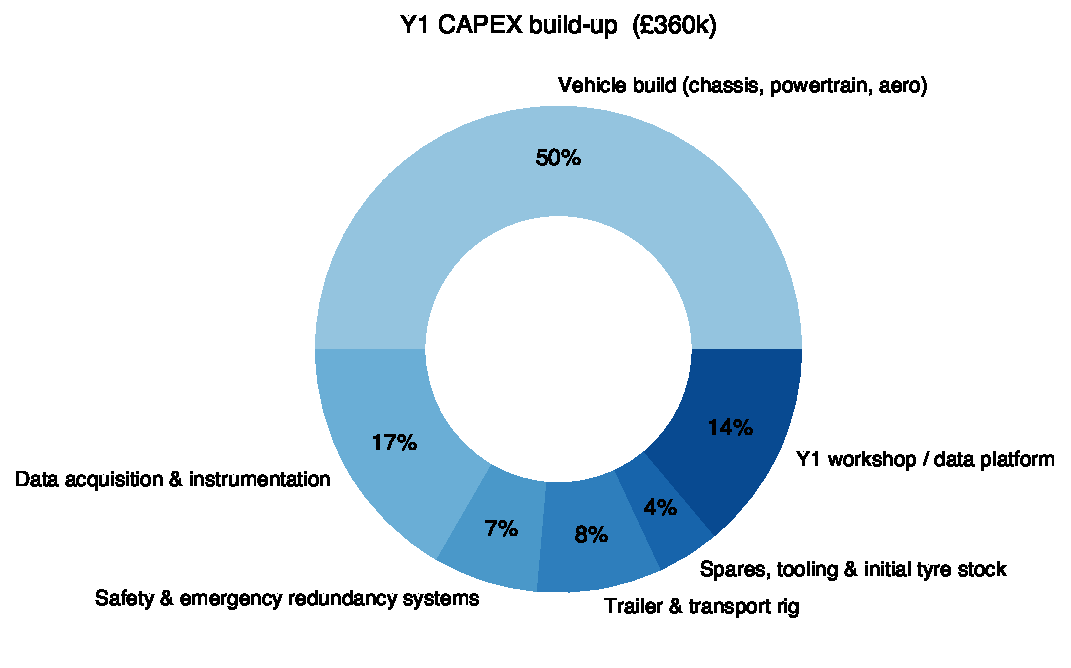
\includegraphics[width=0.92\textwidth,height=0.40\textheight,keepaspectratio]{cost_structure_capex.pdf}
\caption{Y1 CAPEX build-up: per-vehicle line items plus the one-off
  workshop and data-platform setup (same totals as
  Table~\ref{tab:capex_schedule}, Y1 column).}
\label{fig:capex_donut}
\end{figure}

Capital is depreciated on a five-year straight-line basis. No
residual value is modelled at Y5: in a PSS business, the physical
asset is either refurbished in place following the 9R lifecycle loop (see the 9R framework discussion earlier in this report)---and therefore stays in service beyond the modelled window---or is
retired in line with safety-critical-testing industry norms.

\begin{table}[H]
\centering
\small
\caption{Five-year capex schedule (\pounds k). Per-vehicle build costs 
\pounds310k (component split in Figure~\ref{fig:capex_donut}); 
one-off Y1 company setup \pounds50k.}
\label{tab:capex_schedule}
\begin{tabular}{cccccc}
\toprule
\textbf{Year} & \textbf{New vehicles} & \textbf{Vehicle capex} & \textbf{Other capex} & \textbf{Total} \\
\midrule
1 & 1 & 310 & 50 & \textbf{360} \\
2 & 0 & 0 & 0 & \textbf{0} \\
3 & 1 & 310 & 0 & \textbf{310} \\
4 & 0 & 0 & 0 & \textbf{0} \\
5 & 1 & 310 & 0 & \textbf{310} \\
\bottomrule
\end{tabular}
\end{table}


% ---------------------------------------------------------------------
\subsection{OPEX model: a fixed-cost-heavy delivery operation}
\label{sec:opex}
% ---------------------------------------------------------------------

\begin{figure}[H]
\centering
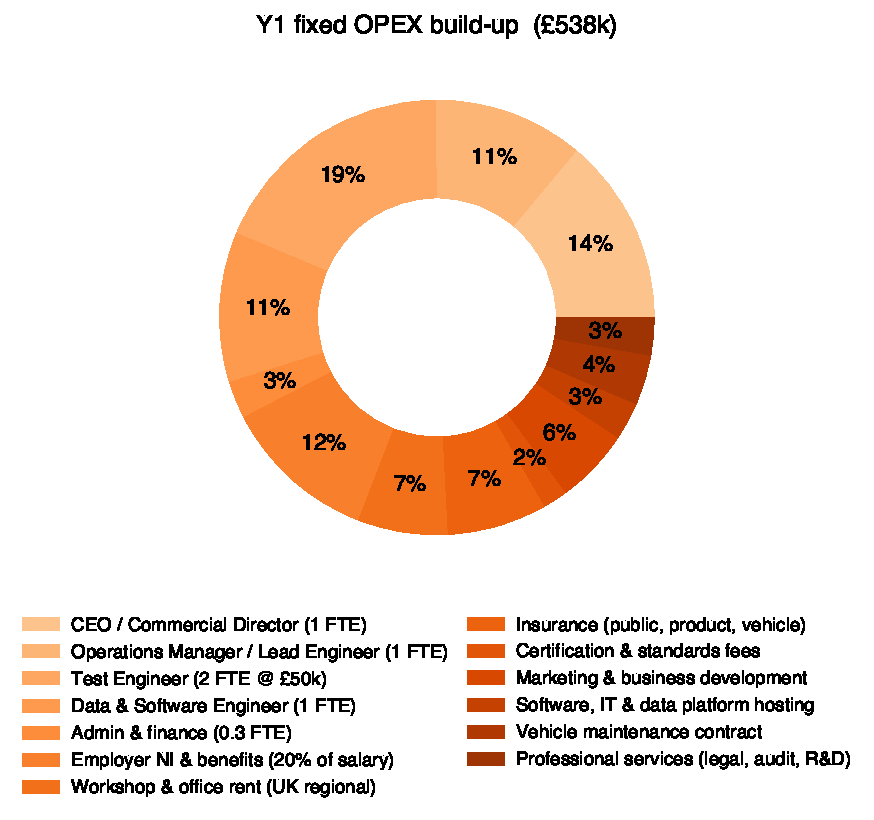
\includegraphics[width=0.92\textwidth,height=0.44\textheight,keepaspectratio]{cost_structure_opex.pdf}
\caption{Y1 fixed-OPEX build-up. Legend in two columns for legibility.
  The salary-heavy stack is the reason utilisation (revenue per
  engineer per year) is the highest-leverage financial driver in
  the sensitivity analysis (Section~\ref{sec:business_sensitivity}).}
\label{fig:opex_donut}
\end{figure}

\noindent Fixed opex is dominated by headcount (60\% of the Y1 opex base of
\fixedOpexYOne), with the remainder split across workshop rent,
insurance, certification fees, data-platform hosting, marketing,
vehicle maintenance, and professional services.
The model inflates fixed opex at 3\% per year (UK CPIH 2023--25 trend) and
adds step-changes for each fleet-growth hire.

Variable cost per test day is \pounds2,300 (Y1), comprising tyres
and consumables (\pounds800), transport (\pounds600), crew
travel-and-subsistence (\pounds400), and amortised vehicle wear
(\pounds500). The resulting contribution margin per test day is
\contributionMargin at Y2 -- this is the single number that drives
the break-even analysis below.

% ---------------------------------------------------------------------
\subsection{Revenue model: every pound tethered to fleet utilisation}
\label{sec:revenue}
% ---------------------------------------------------------------------

Revenue is modelled bottom-up from three driver arrays: test days
sold, fleet size, and blended day-rate. Day-rate is the
mix-weighted average of the Bronze / Silver / Gold packages
(\pounds6\,k / \pounds8\,k / \pounds10\,k) benchmarked against
the competitor set discussed in the competitive landscape analysis earlier in this report
(AB~Dynamics~\cite{abdynamics_ar2024},
UTAC~\cite{utac_facilities},
HORIBA~\cite{horiba_brake}, and AVL~\cite{avl_profile}). Mix-shift
from Bronze-heavy to Gold-heavy over five years drives blended
day-rate from \pounds7.5\,k (Y1) to \pounds9.5\,k (Y5) without
any individual-tier price movement -- important for the pricing
discipline discussed in Section~\ref{sec:business_sensitivity}.

\begin{table}[H]
\centering
\small
\caption{Revenue build-up: test days, fleet utilisation, blended day 
rate, and resulting gross-profit stack.}
\label{tab:revenue}
\begin{tabular}{lrrrrr}
\toprule
\textbf{Metric} & \textbf{Y1} & \textbf{Y2} & \textbf{Y3} & \textbf{Y4} & \textbf{Y5} \\
\midrule
Test days sold & 40 & 70 & 110 & 150 & 220 \\
Fleet size & 1 & 1 & 2 & 2 & 3 \\
Utilisation (days/vehicle) & 40 & 70 & 55 & 75 & 73 \\
Blended day rate (\pounds) & 7,500 & 8,000 & 8,500 & 9,000 & 9,500 \\
Revenue (\pounds k) & 300 & 560 & 935 & 1,350 & 2,090 \\
Variable cost (\pounds k) & 92 & 164 & 264 & 368 & 550 \\
Gross profit (\pounds k) & 208 & 396 & 671 & 982 & 1,540 \\
Gross margin (\%) & 69.3 & 70.6 & 71.8 & 72.8 & 73.7 \\
\bottomrule
\end{tabular}
\end{table}


\paragraph{Reconciliation with market sizing.}
Y5 forecast revenue of \yFiveRevenue ($\approx$\textdollar 2.7\,M)
sits at \mbox{10--14\%} of the serviceable-obtainable-market estimate
(\textdollar 26\,M) from that market-sizing analysis -- a
penetration consistent with a credible early-stage entrant, with
upside if utilisation and mix outperform the base plan.

% ---------------------------------------------------------------------
\subsection{Five-year profit \& loss forecast}
\label{sec:pnl}
% ---------------------------------------------------------------------

Table~\ref{tab:pnl} is the five-year P\&L summary; every column is
a downstream result of the cost and revenue models above. Three
features are worth noting:

\begin{tightitemize}
  \item \textbf{EBITDA turns positive in Y4}, well before net
        profit, reflecting the drag of depreciation in a
        capex-heavy service business.
  \item \textbf{Operating-leverage tipping point at Y3.} Gross
        profit grows faster than fixed opex from Y3 onwards;
        Y3 is the \emph{commercial} break-even year, Y4 is the
        \emph{accounting} break-even year.
  \item \textbf{Corporation tax kicks in at Y4} (UK small-profits
        rate 19\% in the 2025/26 regime). The Y5 net profit
        of \pounds293\,k is reported after tax.
\end{tightitemize}

\begin{table}[H]
\centering
\small
\caption{Five-year P\&L summary (\pounds k). All figures flow from 
the single driver set stated in Sections~\ref{sec:capex}--\ref{sec:revenue}.}
\label{tab:pnl}
\begin{tabular}{lrrrrr}
\toprule
\textbf{Line} & \textbf{Y1} & \textbf{Y2} & \textbf{Y3} & \textbf{Y4} & \textbf{Y5} \\
\midrule
Revenue & 300 & 560 & 935 & 1,350 & 2,090 \\
Variable cost & -92 & -164 & -264 & -368 & -550 \\
Gross profit & 208 & 396 & 671 & 982 & 1,540 \\
Fixed opex & -538 & -616 & -693 & -834 & -983 \\
EBITDA & -330 & -220 & -22 & 149 & 557 \\
Depreciation & -72 & -72 & -134 & -134 & -196 \\
EBIT & -402 & -292 & -156 & 15 & 361 \\
Tax @ 19\% & -0 & -0 & -0 & -3 & -69 \\
Net profit & -402 & -292 & -156 & 12 & 293 \\
\bottomrule
\end{tabular}
\end{table}


\begin{figure}[H]
\centering
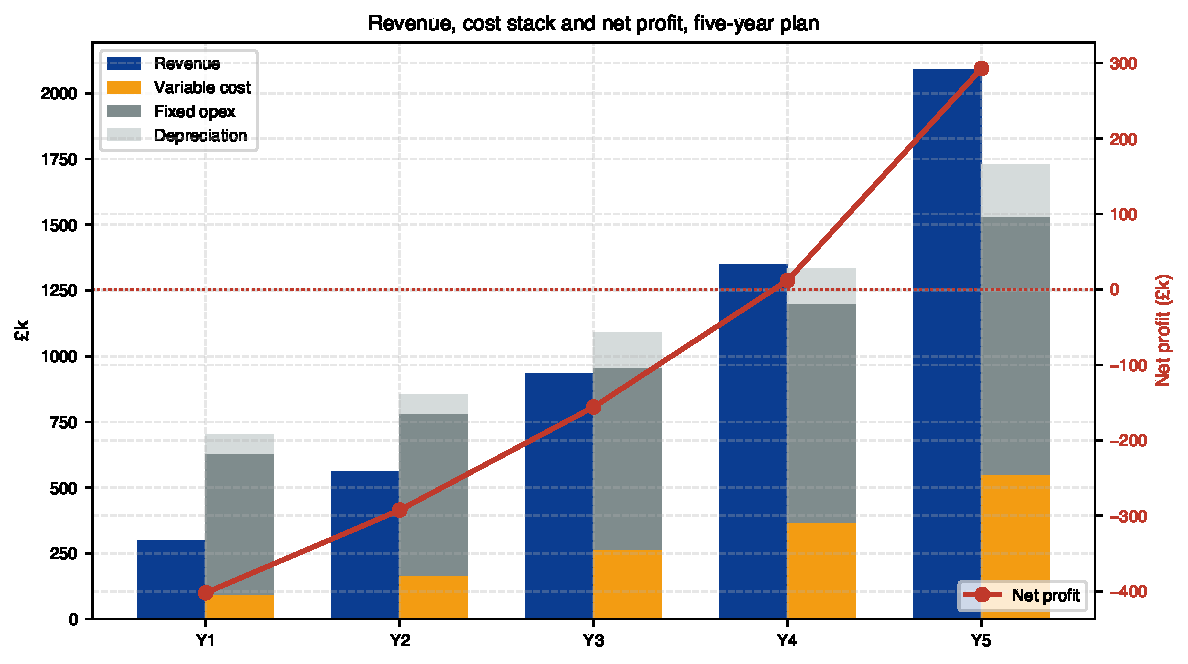
\includegraphics[width=\textwidth]{revenue_ramp.pdf}
\caption{Five-year revenue (blue) against the full cost stack
  (variable, fixed, depreciation) with net-profit trajectory
  overlaid (red, right axis). Net profit crosses zero in Y4 --
  the accounting break-even year -- and reaches \pounds293\,k
  net of tax in Y5.}
\label{fig:revenue_ramp}
\end{figure}

% ---------------------------------------------------------------------
\subsection{Five-year cash-flow forecast}
\label{sec:cash_flow}
% ---------------------------------------------------------------------

A capex-heavy TaaS business lives or dies on cash, not on
accounting profit. Figure~\ref{fig:cash} summarises free cash flow,
equity raises, and cumulative cash balance.

\begin{figure}[H]
\centering
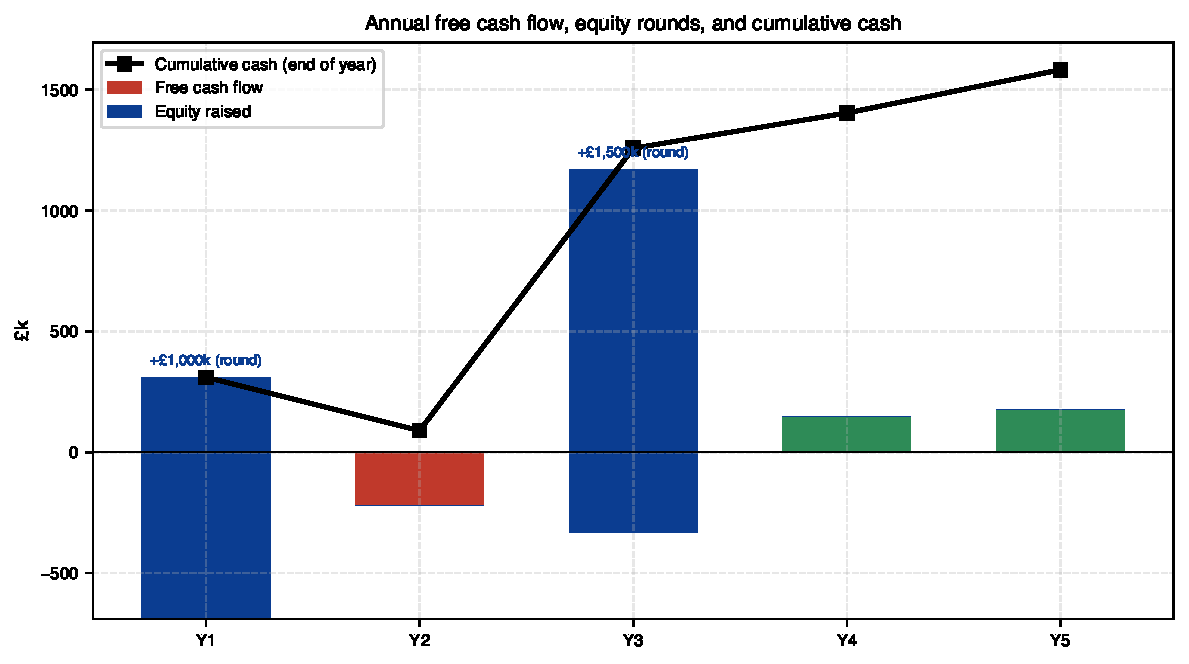
\includegraphics[width=\textwidth]{cash_waterfall.pdf}
\caption{Annual free cash flow (green/red bars), equity rounds
  (blue stacked bars), and cumulative cash balance (black line).
  Cumulative cash reaches its minimum of \pounds90\,k at end-Y2 --
  the trigger point for Series~A close -- and turns structurally
  positive from Y3 onwards once the Series~A has closed.}
\label{fig:cash}
\end{figure}

Two moments deserve attention. First, end-Y2 cash balance is
\pounds90\,k -- the tightest point in the plan, after absorbing
two years of operating loss. A delayed Series~A would push the
company into a bridge-round conversation; the Series~A
therefore targets a Q4-Y2 close rather than a Y3 close.
Second, Y5 free cash flow is \pounds179\,k positive even after the
\capexPerVehicle third-vehicle purchase -- the plan is genuinely
self-funding by Y5.

% =====================================================================
\section{Capital-budgeting assessment}
\label{ch:be_npv}
% =====================================================================

% ---------------------------------------------------------------------
\subsection{Break-even analysis}
\label{sec:breakeven}
% ---------------------------------------------------------------------

Break-even on the Y2 fixed-cost base occurs at \breakEvenDays test
days per year. This is the number of days the fleet must sell
annually to cover fixed opex and depreciation:

\begin{equation}
\mathrm{BE_{days}} \;=\; \frac{F + D}{p_{\mathrm{day}} - c_{\mathrm{var}}}
\end{equation}

\noindent where $F$ is annual fixed opex, $D$ annual depreciation,
$p_{\mathrm{day}}$ the Y2 blended day-rate, and $c_{\mathrm{var}}$
the Y2 variable cost per day. The resulting contribution margin
per day is \contributionMargin; fixed costs plus depreciation total
\pounds690\,k~Y2.

\begin{figure}[H]
\centering
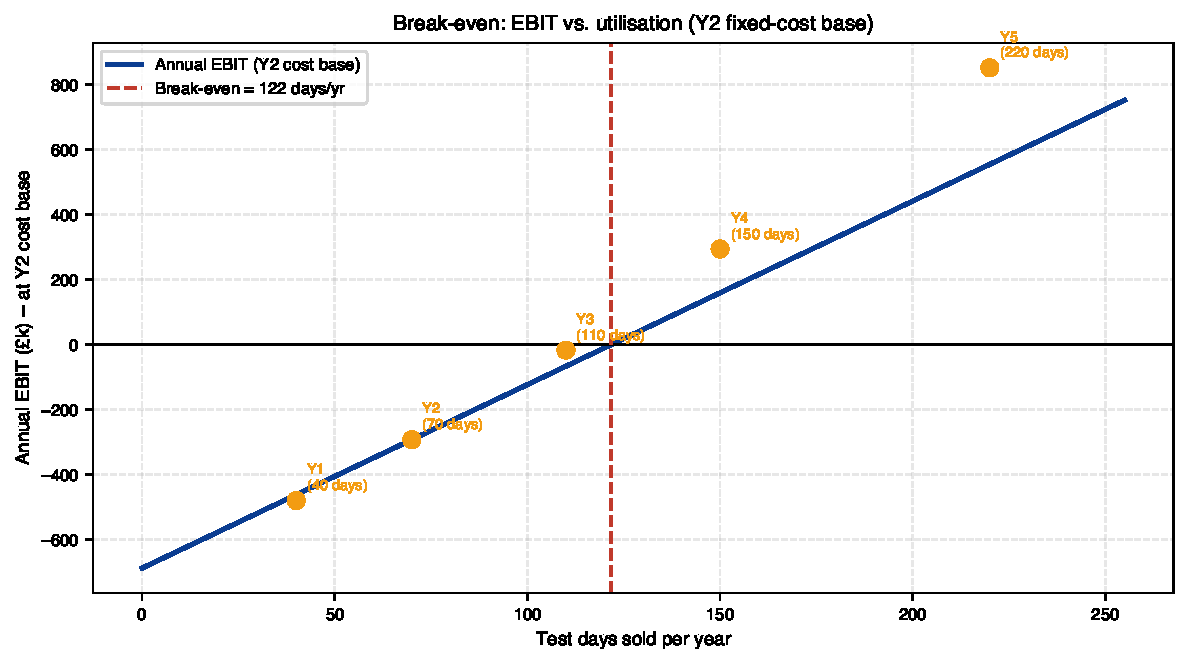
\includegraphics[width=\textwidth]{break_even.pdf}
\caption{Break-even curve -- annual EBIT at the Y2 cost base as a
  function of annual test days. The vertical red dashed line marks
  the \breakEvenDays-day break-even point; orange markers show the
  plan's Y1--Y5 planned utilisation trajectory.}
\label{fig:break_even}
\end{figure}

Y1--Y3 sit below break-even (as expected for an early-stage TaaS
build-out); Y4 is above; Y5 is comfortably above. The gap between
the \breakEvenDays-day requirement and the Y1 plan of 40 days is
the explicit financial quantification of the ``TaaS burden''
period when cumulative CAPEX runs ahead of cumulative revenue in the early ramp.

% ---------------------------------------------------------------------
\subsection{NPV and IRR -- the capital-budgeting view}
\label{sec:npv}
% ---------------------------------------------------------------------

Because the five-year operational FCFs are loss-making until Y4,
accounting profit is an insufficient test of investability. The
appropriate test is discounted cash flow~\cite{brealey2020}:
can the project, including its terminal value, return more than the
investor's hurdle rate?

\paragraph{Method.} Free cash flows (pre-equity, post-CAPEX) are
the annual series underlying Figure~\ref{fig:cash}. A terminal value is added to
Y5 at the peer-group median EV/Revenue multiple of $2.5\times$
Y5 revenue~\cite{abdynamics_ar2024,damodaran2012}, yielding
\terminalValue. The project NPV at a discount rate $r$ is then

\begin{equation}
\mathrm{NPV}(r) \;=\; \sum_{t=1}^{5} \frac{\mathrm{FCF}_t}{(1 + r)^t} \;+\; \frac{\mathrm{TV}}{(1 + r)^5}.
\end{equation}

\noindent The project IRR is the discount rate at which NPV$=0$.

\paragraph{Result.} Figure~\ref{fig:npv} plots $\mathrm{NPV}(r)$
at representative hurdle rates (same annual FCF series as
Figure~\ref{fig:cash}, pre-equity post-CAPEX, plus the Y5
terminal value stated in the Method paragraph). At the 20\%
VC-central rate the project NPV is \npvBase; at the 25\%
high-hurdle rate it is \npvHurdle; IRR is \irr.

\begin{figure}[H]
\centering
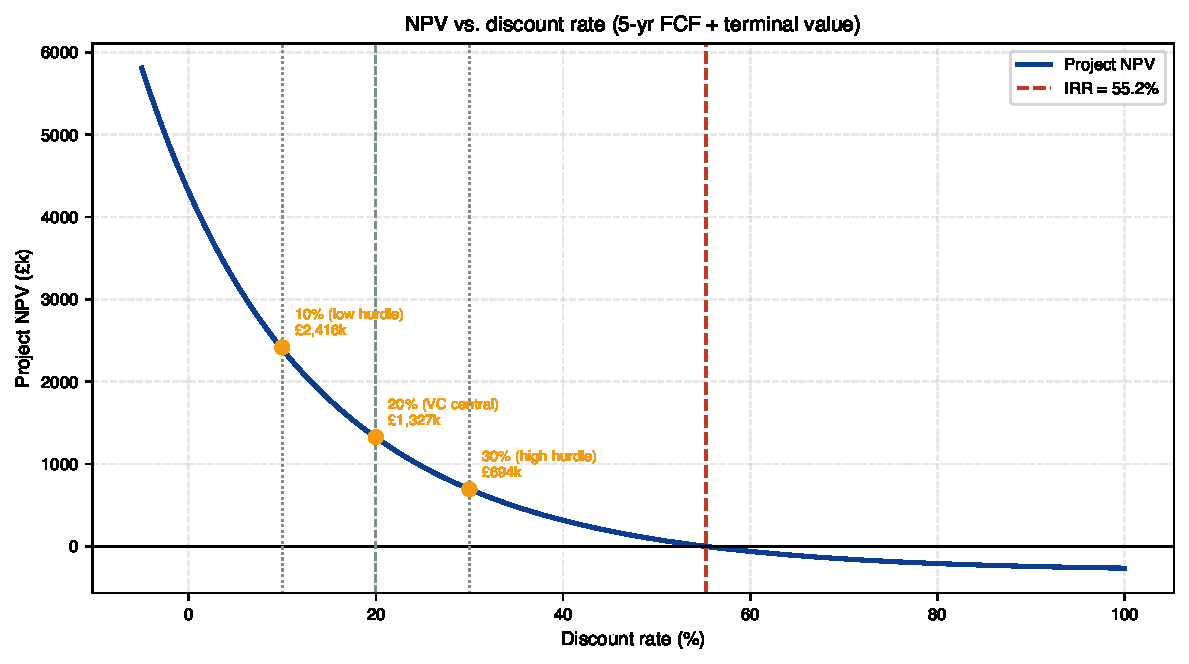
\includegraphics[width=\textwidth]{npv_curve.pdf}
\caption{Project NPV as a function of discount rate $r$. Cash flows
  are the five-year free-cash-flow series underlying
  Figure~\ref{fig:cash} plus terminal value \terminalValue{} at
  $2.5\times$ Y5 revenue (peer-group EV/Revenue median). The 10\% /
  20\% / 30\% hurdle points are annotated; the IRR (\irr) is
  marked with the red vertical dashed line. NPV remains positive
  at discount rates well above typical VC hurdles, driven by the
  present value of the Y5 terminal value.}
\label{fig:npv}
\end{figure}

\paragraph{Interpretation.} The project clears standard VC-hurdle
tests comfortably. Two caveats apply. First, \textbf{almost all
of the NPV is present-value terminal value}, not operational cash
flow: at 20\% the PV of the \terminalValue terminal alone is
\pounds2.1\,M, against \pounds0.8\,M of negative PV from the Y1--Y3
cash outflows. NPV is therefore only as robust as the
exit-multiple assumption. Second, the \irr IRR reflects that a
TaaS project that turns cash-positive in Y5 is, arithmetically, a
very-high-return asset if it can be sold at the terminal multiple;
it does not imply year-by-year operating returns at that level.

% ---------------------------------------------------------------------
\subsection{Sensitivity analysis}
\label{sec:business_sensitivity}
% ---------------------------------------------------------------------

Following the one-at-a-time methodology of the engineering
chapter's sensitivity ranking~\cite{emes_engineering}, each driver
is perturbed by $\pm 20\%$ ($\pm 50\%$ for inflation) and the
resulting Y3 EBIT swings ranked in Figure~\ref{fig:business_tornado}.

\begin{figure}[H]
\centering
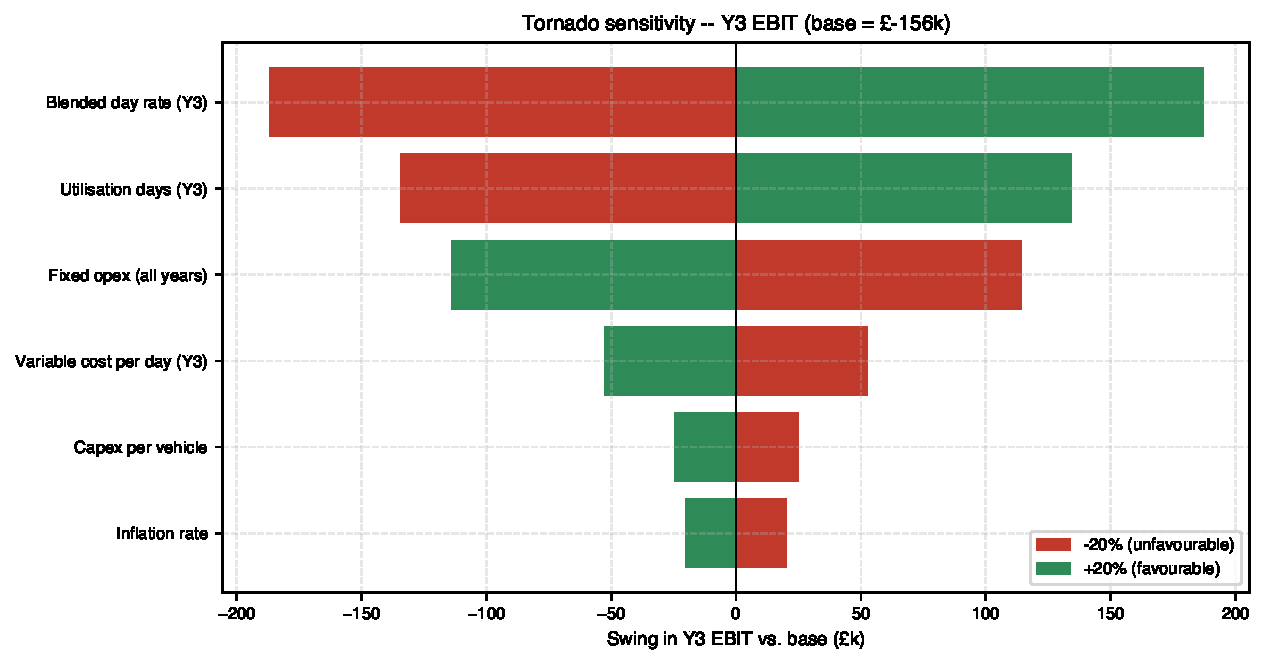
\includegraphics[width=\textwidth]{tornado.pdf}
\caption{Tornado sensitivity of Y3 EBIT to $\pm 20\%$ (or
  $\pm 50\%$) perturbation of each driver. Blended day-rate and
  utilisation dominate; fixed opex is second-order; CAPEX and
  inflation are third-order.}
\label{fig:business_tornado}
\end{figure}

Two implications follow. First, \textbf{pricing discipline matters
more than cost discipline}: a 20\% day-rate swing is worth
\pounds374\,k of Y3 EBIT whereas a 20\% fixed-opex swing is worth
\pounds228\,k. Second, the two top drivers (day-rate and
utilisation) are the two most directly in the operating team's
control -- management attention earns the highest marginal return
there, rather than on cost-out or CAPEX engineering.

% ---------------------------------------------------------------------
\subsection{Scenario analysis}
\label{sec:scenarios}
% ---------------------------------------------------------------------

\begin{figure}[H]
\centering
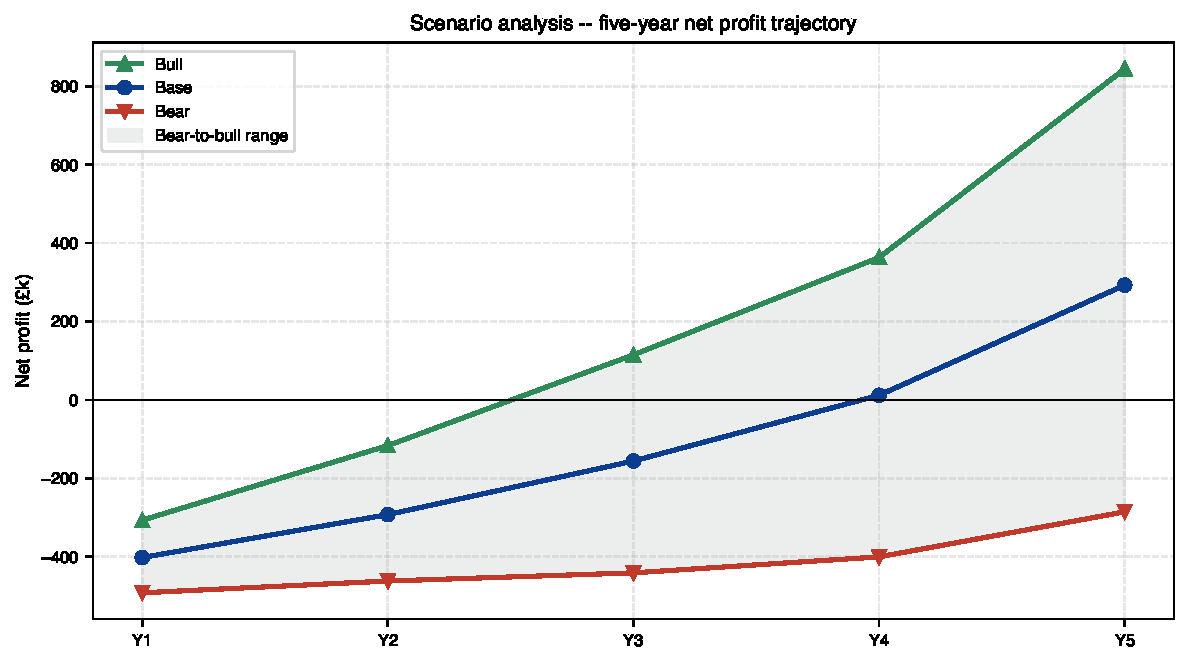
\includegraphics[width=\textwidth]{scenarios.pdf}
\caption{Scenario net-profit after tax (\pounds k, Y1--Y5). Bull reaches
  $+$\pounds844\,k by Y5; Bear stays loss-making ($-$\pounds285\,k)
  and would force a cost reset or bridge financing.}
\label{fig:scenarios}
\end{figure}

Section~\ref{sec:business_sensitivity} varies one driver at a time; Bull and
Bear add two compound cases that stress correlated downside/upside on the two
dominant levers (days and blended rate), bracketing the Base plan developed in
Sections~\ref{sec:capex}--\ref{sec:cash_flow}:

\noindent
\begin{tabular}{@{}>{\raggedright\arraybackslash}p{0.47\textwidth}>{\raggedright\arraybackslash}p{0.47\textwidth}@{}}
\textbf{Bull:} $+25\%$ days, $+10\%$ rate, $-5\%$ variable cost. &
\textbf{Bear:} $-30\%$ days, $-10\%$ rate, $+10\%$ variable cost (heavier than Bull: fixed-cost drag amplifies revenue miss). \\
\end{tabular}

Bear is not a venture-sustainable path: cumulative loss exceeds the
\totalRaise{} equity stack. Bull needs \emph{both} higher volume and
higher pricing---single-driver upside cannot reproduce it
(Figure~\ref{fig:business_tornado}).

% ---------------------------------------------------------------------
\subsection{Minimum viable Commercial conditions}
\label{sec:mvc_conditions}
% ---------------------------------------------------------------------

The Base case in Sections~\ref{sec:revenue}--\ref{sec:cash_flow} shows that
Testing-as-a-Service can reach net profitability within the five-year horizon,
but the path is narrow: a small set of operating and commercial \emph{floors}
defines where the model stops being financeable regardless of optimistic
market growth. This subsection states those \textbf{minimum viable commercial
conditions (MVC)} as thresholds \emph{consistent with the published financial
model} (Table~\ref{tab:revenue}; Figures~\ref{fig:break_even},
\ref{fig:business_tornado}, and \ref{fig:downtime}).

\paragraph{Dominant levers.}
Commercial feasibility is pinned by three linked drivers already encoded in
the revenue build:
\begin{tightitemize}
  \item \textbf{Billable test-days} (fleet utilisation sold to customers),
  \item \textbf{Blended achieved day-rate} (Bronze / Silver / Gold mix
        in Section~\ref{sec:revenue}),
  \item \textbf{Billable-day capture after downtime} (unplanned loss of sold
        days while fixed crew and overhead continue).
\end{tightitemize}
Because most of the operating cost base is fixed or stepped with hires,
profitability and runway are highly sensitive to keeping productive deployment
high \emph{and} predictable (Section~\ref{sec:breakeven}).

\paragraph{Utilisation / day throughput.}
On the Year~2 fixed-cost base (fixed opex plus depreciation totalling
$\sim$\pounds690\,k), EBIT break-even is \breakEvenDays{} sold test-days per
year at the Y2 blended rate and variable cost---the vertical marker in
Figure~\ref{fig:break_even}. Against a notional \textbf{220-day} selling
calendar with \textbf{one} vehicle on the Y2 stack, that implies a load factor
of about \textbf{55\%} ($122/220$). The Base ramp is 40/70/110/150/220 annual
sold days (Table~\ref{tab:revenue}); Years~1--3 sit \textbf{below} that EBIT
break-even by design, which is why equity runway and Series~A timing matter
(Section~\ref{sec:cash_flow}).

\paragraph{Minimum sustainable pricing.}
The published model does \textbf{not} price services in the
$\pounds3$--$\pounds4$\,k/day range; that band is inconsistent with the
benchmarked Bronze/Silver/Gold positioning (\pounds6\,k / \pounds8\,k /
\pounds10\,k) and the Y1--Y5 blended ladder from \pounds7.5\,k to
\pounds9.5\,k (Table~\ref{tab:revenue}). The break-even identity in
Section~\ref{sec:breakeven} uses an \pounds8\,k Y2 blended rate with
\pounds2{,}350 variable cost per day, giving \contributionMargin{} contribution
per day. Figure~\ref{fig:business_tornado} shows day-rate and utilisation
dominate early margins; sustained discounting far below the published ladder
therefore erodes the same buffer that must carry the tight end-Y2 cash
position before any reliance on terminal value.

\paragraph{Reliability / downtime.}
Downtime is modelled as a proportional loss of otherwise planned billable days;
fixed cost does not flex with outages (Section~\ref{sec:downtime}). In that
shock, \textbf{Y5 EBIT turns negative at $\sim$20\%} systematic downtime;
NPV@20\% still has a thin positive tail at very high downtime only if the exit
multiple is unchanged. A practical MVC is therefore to hold unplanned downtime
\textbf{well below the $\sim$20\%} region in Figure~\ref{fig:downtime}, with
\textbf{$<$30-minute recovery} maintained as the engineering assumption that
underpins Table~\ref{tab:revenue}.

\paragraph{Customer concentration / pipeline.}
The Series~A gate in Section~\ref{sec:funding} is explicit:
$\geq$\pounds400\,k ARR and \textbf{at least two} retainer customers. Y1 sells
only 40 days; using the same unit-economics illustration as the LTV block
($\sim$8 test days per customer-year at \pounds7.5\,k;
Section~\ref{sec:funding}), that implies \textbf{order five} active commercial
relationships at Base intensity---not a portfolio of one-off micro-projects.
Section~\ref{sec:cash_risk} already flags $>$30\% of Y1 revenue from a single
pilot; widening beyond that concentration is part of the MVC, not an optional
nice-to-have.

\paragraph{Capital structure.}
The published Base is \textbf{equity-funded}: \totalRaise{} (\seedRound{} seed
plus \seriesARound{} Series~A) with \totalCapex{} phased vehicle additions per
Table~\ref{tab:revenue}. No term debt is layered into the cash forecasts;
adding leverage would tighten the end-Y2 \pounds90\,k headroom without changing
the utilisation arithmetic. The MVC financing configuration is therefore
\textbf{phased fleet expansion on equity}, not debt-funded scaling before
utilisation is proven.

\paragraph{Correlated downside (joint stress).}
Section~\ref{sec:scenarios} stresses that single-variable optimism is not
enough: if sold days, blended rate, and variable \pounds/day move \emph{together}
toward the Bear profile, NPV@20\% crosses zero at about \textbf{four-fifths} of
that joint move, with only ${<}$\pounds100\,k of Y5 net separating the NPV
knife-edge from the Bear outcome (Figure~\ref{fig:scenarios}). Treat sustained
simultaneous deterioration on all three levers as a capital trigger tracked
through the KPI pack in Section~\ref{sec:valuation}.

\begin{table}[H]
\centering
\caption{Minimum viable commercial conditions---summary aligned to the Base
  financial model.}
\label{tab:mvc_summary}
\begin{tabular}{p{5.0cm}p{9.0cm}}
\hline
\textbf{Parameter} & \textbf{Condition (per Base model)} \\
\hline
Sold test-days (Y2 EBIT break-even) &
  $\geq$ \breakEvenDays{} billable days/year at the Y2 rate/cost stack
  (Figure~\ref{fig:break_even}). \\
Planned utilisation ramp &
  Deliver the Base ladder 40/70/110/150/220 annual sold days
  (Table~\ref{tab:revenue}). \\
Blended day-rate &
  Stay on the published \pounds7.5\,k--\pounds9.5\,k trajectory; tier floor
  in positioning is Bronze at \pounds6\,k (Section~\ref{sec:revenue}). \\
Unplanned downtime &
  Hold systematic loss of billable days $\ll \sim$20\%; keep the
  fast-recovery operating assumption in Section~\ref{sec:downtime}. \\
Series~A commercial gate &
  $\geq$\pounds400\,k ARR and $\geq$2 retainer customers
  (Section~\ref{sec:funding}). \\
Y1 relationship depth (indicative) &
  Order $\sim$5 active customers at the $\sim$8 days/customer-year load used
  in Section~\ref{sec:funding}; diversify away from single-pilot dependence
  (Section~\ref{sec:cash_risk}). \\
Financing &
  Equity as published (\totalRaise{}); do not rely on debt against
  utilisation-linked early cash. \\
\hline
\end{tabular}
\end{table}

\noindent\textbf{Take-away.} In this chapter, long-term viability depends less
on extreme technical heroics and more on \textbf{repeatable billable-day
delivery} at the rates, downtime, and funding assumptions already embedded in
the model.

% =====================================================================
\section{Financial risk: the downtime case}
\label{ch:risk_fin}
% =====================================================================

Industry-level risks are covered earlier in this report in the dedicated strategic-risk analysis.
Here the focus is financial: if fleet maintenance fails
operationally, how much do NPV and EBIT suffer? For TaaS, revenue follows
utilisation (Section~\ref{sec:why_taas}), so that maintenance risk is the
main execution risk.

% ---------------------------------------------------------------------
\subsection{Downtime sensitivity -- quantifying the maintenance dependency}
\label{sec:downtime}
% ---------------------------------------------------------------------

Following the supply-chain planning framework introduced earlier in this report, we assume
$<$30-minute fleet recovery from any single failure; this underpins the
planned utilisation arrays in Table~\ref{tab:revenue}. Downtime is modelled
as a fractional reduction in billable days: a downtime rate of
$d\%$ delivers $(1-d)\cdot D_t$ billable days in year $t$. The fixed
cost base is unchanged (the crew is still paid while the vehicle is
grounded), so every percentage point of downtime translates
one-for-one into lost gross profit.

\begin{figure}[H]
\centering
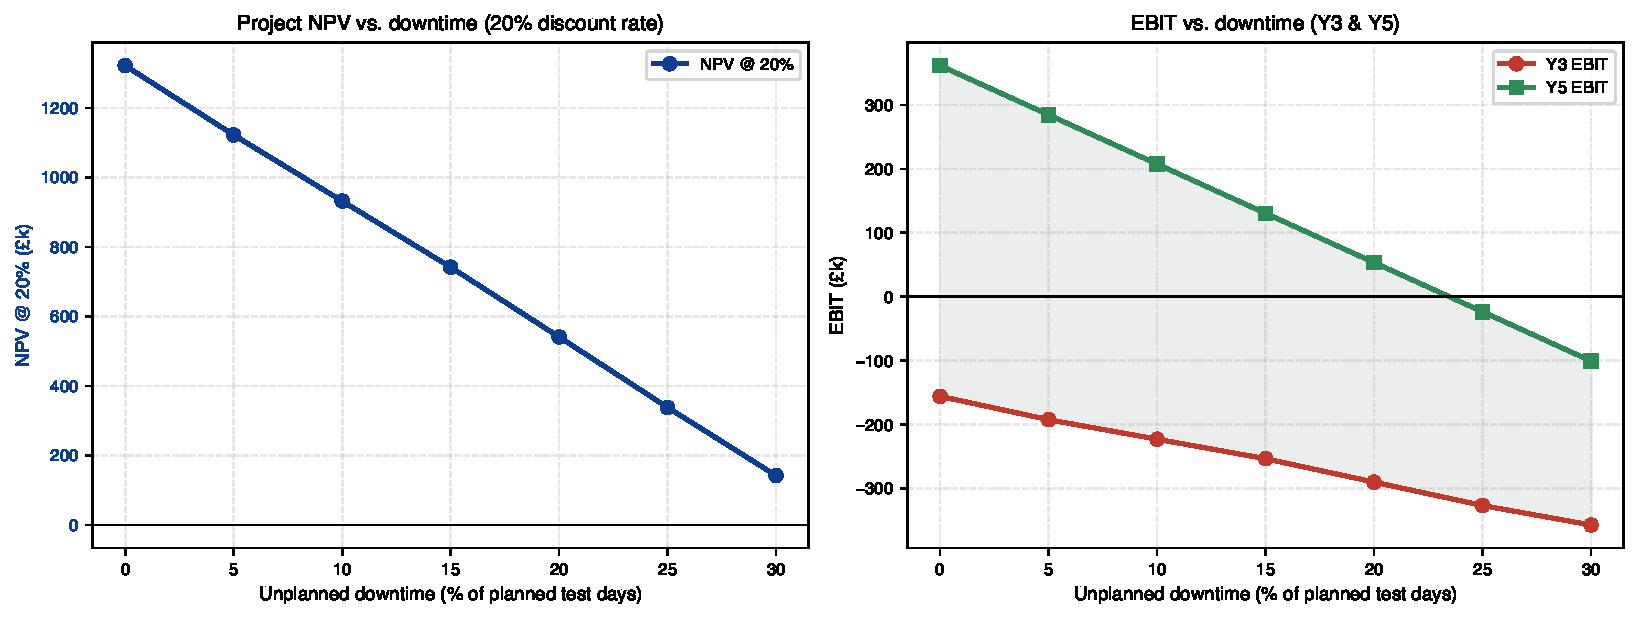
\includegraphics[width=\textwidth]{downtime.pdf}
\caption{Downtime sensitivity. Left: project NPV at 20\%
  discount rate as a function of unplanned downtime; NPV stays
  positive through \downtimeBreak downtime, with the residual
  value dominated by the terminal contribution at high downtime.
  Right: Y3 (red) and Y5 (green) EBIT for the same shock; Y5 EBIT
  turns negative at $\sim$20\% downtime, illustrating that
  operating earnings deteriorate before NPV exhausts its margin.}
\label{fig:downtime}
\end{figure}

\paragraph{Interpretation.}
\begin{tightitemize}
  \item \textbf{EBIT is brittle.} Y3 EBIT deteriorates from
        $-$\pounds156\,k to $-$\pounds357\,k as downtime rises
        from 0 to 30\%; Y5 EBIT turns negative at $\sim$20\%
        downtime.
  \item \textbf{NPV is less brittle -- but only as long as the
        exit multiple holds.} NPV@20\% falls from
        \pounds1.32\,M to \pounds0.14\,M at 30\% downtime, still
        positive but with little margin. If the downtime event
        also compresses the exit multiple
        (acquirers discount unreliability), NPV can flip negative
        at lower downtime levels.
  \item \textbf{Maintenance is cheap to fund but expensive to starve.}
        Relative to the recurring maintenance cash costs in the base plan,
        the losses from systematic downtime dominate: at 10\% downtime,
        \pounds190\,k of Y5 revenue, \pounds154\,k of Y5 EBIT, and
        \pounds390\,k of NPV@20\% are lost; at 20\% downtime those figures
        rise to \pounds418\,k, \pounds308\,k, and \pounds781\,k.
\end{tightitemize}

\paragraph{Implication for the maintenance budget.} The financial
cost of a 10\% systematic downtime (\pounds390\,k NPV reduction) is
more than double the total Y1 vehicle-maintenance contract
(\pounds20\,k) and an order of magnitude above the incremental
cost of a spare-vehicle strategy. Investment in maintenance
capability should be benchmarked against this NPV-protection
value, not the headline opex line.

% ---------------------------------------------------------------------
\subsection{Financial risk: cash-headroom assessment}
\label{sec:cash_risk}
% ---------------------------------------------------------------------

The cash forecast (Section~\ref{sec:cash_flow}) identified
end-Y2 cash balance of \pounds90\,k as the tightest point of the
plan. A compounded shock at that moment -- for example, a
Series~A close three months late plus a reportable safety
incident -- is sufficient to push the business into bridge-round
territory. Three specific financial exposures follow:

\begin{tightitemize}
  \item \textbf{Series~A timing.} Only \pounds90\,k buffer at
        Y2/Y3 boundary. Series~A prep therefore starts at Month~15
        to target a Q4-Y2 close; bridge-round authorisation is
        pre-negotiated with seed investors in the seed term sheet.
  \item \textbf{Reportable safety incident.} A single incident can
        increase insurance premium by $2$--$5\times$ (shifting the
        insurance line from $\sim$\pounds20\,k/year to
        $\sim$\pounds50--100\,k/year) and close the OEM
        supplier-approval pathway -- gating the
        Phase~3~Y4+ revenue ramp.
  \item \textbf{Anchor-customer concentration.} In Y1,
        $>$30\% of revenue is from a single pilot customer. The
        Series~A trigger therefore requires \emph{two} retainer
        conversions, not one, to decouple the capital raise from
        single-customer concentration.
\end{tightitemize}

These financial-risk mitigations align with the execution plan but are
framed here as cash outcomes: the industry-level strategic-risk material is
discussed earlier in this report, whereas this subsection adds the
liquidity and runway perspective needed for financial evaluation.

% =====================================================================
\section{Funding strategy, valuation and financial KPIs}
\label{ch:funding}
% =====================================================================

% ---------------------------------------------------------------------
\subsection{Funding strategy and use of funds}
\label{sec:funding}
% ---------------------------------------------------------------------

The plan requires a total of \totalRaise of equity, in two
rounds.

\begin{tightitemize}
  \item \textbf{Seed, \seedRound at incorporation.} Used for Y1
        vehicle build (\capexPerVehicle), Y1 workshop / data-platform
        setup (\pounds50\,k), and $\sim$18 months of runway
        ($\sim$\pounds600\,k). Indicative pre-money valuation
        \pounds4\,M $\Rightarrow$ 20\% equity round.
  \item \textbf{Series~A, \seriesARound at Q4-Y2 / Q1-Y3.} Used
        for the second-vehicle build, Y3--Y4 headcount additions
        (BD/Sales, second test engineer), and a further $\sim$18
        months of runway. Indicative pre-money valuation
        \pounds6\,M $\Rightarrow$ 20\% equity round.
\end{tightitemize}

\noindent The \textbf{Series~A trigger is revenue-based, not
runway-based}: $\geq$\pounds400\,k ARR and $\geq$ 2 retainer
customers. Missing the trigger implies a bridge round from seed
investors rather than a Series~A at a compressed valuation; the
seed term sheet should pre-authorise this bridge.

\medskip

\noindent \textbf{Unit economics.} Using an average customer of
$\sim$8 test days/year at a blended day-rate of \pounds7.5\,k,
three-year average relationship, and 70\% revenue-weighted gross
margin:

\begin{equation}
\mathrm{LTV} = (8 \times 7{,}500) \times 3 \times 0.70 = \ltv,
\qquad
\frac{\mathrm{LTV}}{\mathrm{CAC}} = \ltvCac,
\qquad
\mathrm{Payback} = \paybackMonths \text{ months}.
\end{equation}

Both metrics clear standard B2B-services investability
thresholds~\cite{gompers2020} by a wide margin; a doubling of CAC
still clears the 3$\times$ LTV/CAC rule.

% ---------------------------------------------------------------------
\subsection{Valuation (comparable multiples)}
\label{sec:valuation}
% ---------------------------------------------------------------------

Indicative Y5 valuation uses listed-peer EV/Revenue multiples,
benchmarked against AB~Dynamics (LSE:~ABDP), Spirent Communications
(LSE:~SPT), and AVL~List~\cite{abdynamics_ar2024,avl_profile}.

\begin{table}[H]
\centering
\small
\caption{Comparable-multiples valuation. Year-5 forecast revenue 
(\pounds2.1M) multiplied by peer EV/Revenue multiples 
gives the indicative Year-5 enterprise-value range.}
\label{tab:valuation}
\begin{tabular}{lcr}
\toprule
\textbf{Peer} & \textbf{EV / Revenue} & \textbf{Implied EV (\pounds M)} \\
\midrule
AB Dynamics (LSE: ABDP, 2024) & 3.5$\times$ & 7.3 \\
Spirent Communications (LSE: SPT) & 2.2$\times$ & 4.6 \\
AVL List (private, Refinitiv est.) & 1.8$\times$ & 3.8 \\
Peer-group median & 2.5$\times$ & 5.2 \\
\bottomrule
\end{tabular}
\end{table}


At the peer-group median of $2.5\times$ Y5 revenue, the indicative
Y5 enterprise value is \terminalValue; the AB~Dynamics multiple
(3.5$\times$) yields \pounds7.3\,M. This range bracketed the
terminal-value assumption used in the NPV analysis
(Section~\ref{sec:npv}); the NPV conclusion is robust within this
band but sensitive to a compression below the peer-group floor
(AVL at 1.8$\times$).

% =====================================================================
\section{Conclusions and Recommendations}
\label{ch:concl}
% =====================================================================

The AEB~Rabbit TaaS business clears standard capital-budgeting
thresholds in the base case: project NPV of \npvBase at a 20\%
VC-central discount rate, IRR of \irr, and break-even in
\breakEvenYear at \breakEvenDays test days/year. The financial
structure is typical of a capex-inverted services build-out -- loss
through Y3, cash-thin at the Y2/Y3 boundary, and NPV dominated by
the present value of the Y5 exit. Three recommendations follow, each
paired with the Y1 financial action it drives.

\begin{tightenumerate}
  \item \textbf{Invest ahead of the maintenance-protocol budget.}
        A 10\% systematic downtime costs \pounds390\,k of NPV --
        an order of magnitude above the baseline maintenance-opex
        line. \emph{Y1 action}: scope a spare-vehicle strategy
        and benchmark it against the NPV-protection value, not
        the accounting opex.
  \item \textbf{Prioritise pricing discipline over cost discipline
        in management incentives.} The sensitivity ranking
        identifies blended day-rate as the highest-leverage
        financial driver; the commercial team should be
        compensated on mix-shift to Silver/Gold, not only on
        volume. \emph{Y1 action}: incentive plan pays on blended
        day-rate, not bookings.
  \item \textbf{Protect the Y2/Y3 cash boundary at all costs.}
        Only \pounds90\,k of buffer; compound shocks can
        cascade into a bridge round at a compressed valuation.
        \emph{Y1 action}: target Series~A close at Q4-Y2, not Y3.
\end{tightenumerate}

\medskip

\noindent The TaaS financial structure is viable and
defensible. The single biggest threat to financial returns is not
the external market, the competitors, or the cost base -- it is
the execution of the recovery assumptions in the supply-chain planning framework introduced earlier in this report that the model assumes.
Protecting that assumption is both the cheapest and
highest-leverage financial action the operator can take.

% =====================================================================
\compactbib

\end{refsection}

\end{document}
